\documentclass[
  bibliography=totoc,     % Literatur im Inhaltsverzeichnis
  captions=tableheading,  % Tabellenüberschriften
  titlepage=firstiscover, % Titelseite ist Deckblatt
  12pt,
]{scrartcl}

\usepackage[left=2.5cm, right=2.5cm, top=3.5cm, bottom=3.5cm]{geometry}
\linespread{1.5}

% Paket float verbessern
\usepackage{scrhack}

% Warnung, falls nochmal kompiliert werden muss
\usepackage[aux]{rerunfilecheck}

% % deutsche Spracheinstellungen
% \usepackage[ngerman]{babel}
\usepackage[utf8]{inputenc}
\usepackage[T1]{fontenc}
\usepackage{textcomp}

\usepackage{mathptmx}


% unverzichtbare Mathe-Befehle
\usepackage{amsmath}
% viele Mathe-Symbole
\usepackage{amssymb}
% Erweiterungen für amsmath
\usepackage{mathtools}

% Fonteinstellungen
% \usepackage{fontspec}
% Latin Modern Fonts werden automatisch geladen
% Alternativ zum Beispiel:
%\setromanfont{Libertinus Serif}
%\setsansfont{Libertinus Sans}
%\setmonofont{Libertinus Mono}

% Wenn man andere Schriftarten gesetzt hat,
% sollte man das Seiten-Layout neu berechnen lassen
\recalctypearea{}

% \usepackage[
%   math-style=ISO,    % ┐
%   bold-style=ISO,    % │
%   sans-style=italic, % │ ISO-Standard folgen
%   nabla=upright,     % │
%   partial=upright,   % ┘
%   warnings-off={           % ┐
%     mathtools-colon,       % │ unnötige Warnungen ausschalten
%     mathtools-overbracket, % │
%   },                       % ┘
% ]{unicode-math}

% traditionelle Fonts für Mathematik
% \setmathfont{Latin Modern Math}
% Alternativ zum Beispiel:
%\setmathfont{Libertinus Math}

% \setmathfont{XITS Math}[range={scr, bfscr}]
% \setmathfont{XITS Math}[range={cal, bfcal}, StylisticSet=1]

% Zahlen und Einheiten
\usepackage[
  locale=DE,                   % deutsche Einstellungen
  separate-uncertainty=true,   % immer Fehler mit \pm
  per-mode=symbol-or-fraction, % / in inline math, fraction in display math
]{siunitx}

% chemische Formeln
\usepackage[
  version=4,
  math-greek=default, % ┐ mit unicode-math zusammenarbeiten
  text-greek=default, % ┘
]{mhchem}

% richtige Anführungszeichen
\usepackage[autostyle]{csquotes}

% schöne Brüche im Text
\usepackage{xfrac}

% Standardplatzierung für Floats einstellen
\usepackage{float}
\floatplacement{figure}{htbp}
\floatplacement{table}{htbp}

% Floats innerhalb einer Section halten
\usepackage[
  section, % Floats innerhalb der Section halten
  below,   % unterhalb der Section aber auf der selben Seite ist ok
]{placeins}

% Seite drehen für breite Tabellen: landscape Umgebung
\usepackage{pdflscape}

% Captions schöner machen.
\usepackage[
  labelfont=bf,        % Tabelle x: Abbildung y: ist jetzt fett
  font=small,          % Schrift etwas kleiner als Dokument
  width=0.9\textwidth, % maximale Breite einer Caption schmaler
]{caption}
% subfigure, subtable, subref
\usepackage{subcaption}

% Grafiken können eingebunden werden
\usepackage{graphicx}
% größere Variation von Dateinamen möglich
\usepackage{grffile}

% schöne Tabellen
\usepackage{booktabs}

% Verbesserungen am Schriftbild
\usepackage{microtype}

% Literaturverzeichnis
\usepackage[
  backend=biber,
]{biblatex}
% Quellendatenbank
\addbibresource{lit.bib}
\addbibresource{programme.bib}

% Hyperlinks im Dokument
\usepackage[
  unicode,        % Unicode in PDF-Attributen erlauben
  pdfusetitle,    % Titel, Autoren und Datum als PDF-Attribute
  pdfcreator={},  % ┐ PDF-Attribute säubern
  pdfproducer={}, % ┘
]{hyperref}
% erweiterte Bookmarks im PDF
\usepackage{bookmark}

% Trennung von Wörtern mit Strichen
\usepackage[shortcuts]{extdash}

\setlength{\parskip}{2pt}
\setlength{\parindent}{0pt}
\usepackage{xfrac}
\usepackage{wrapfig}
\usepackage{blindtext}


\subject{Machine Learning for Physicists}
\title{Cloud Classification}

\author{%
  Noah Biederbeck\\%
  \href{mailto:noah.biederbeck@udo.edu}{noah.biederbeck@udo.edu}%
  \texorpdfstring{\and}{,}%
  Maximilian Sackel\\%
  \href{mailto:maximilian.sackel@udo.edu}{maximilian.sackel@udo.edu}%
}
\date{%
  31. Juli 2018
}

\begin{document}

\pagenumbering{roman}
\maketitle
\thispagestyle{empty}
\tableofcontents
\newpage
\nocite{keras}

\pagenumbering{arabic}
\section{Blindtext}\blindtext\blindtext\blindtext
\section{Motivation}
\label{sec:Motivation}

\begin{wrapfigure}{r}{0.43\textwidth}
		\vspace{-0.9cm}
		\centering
		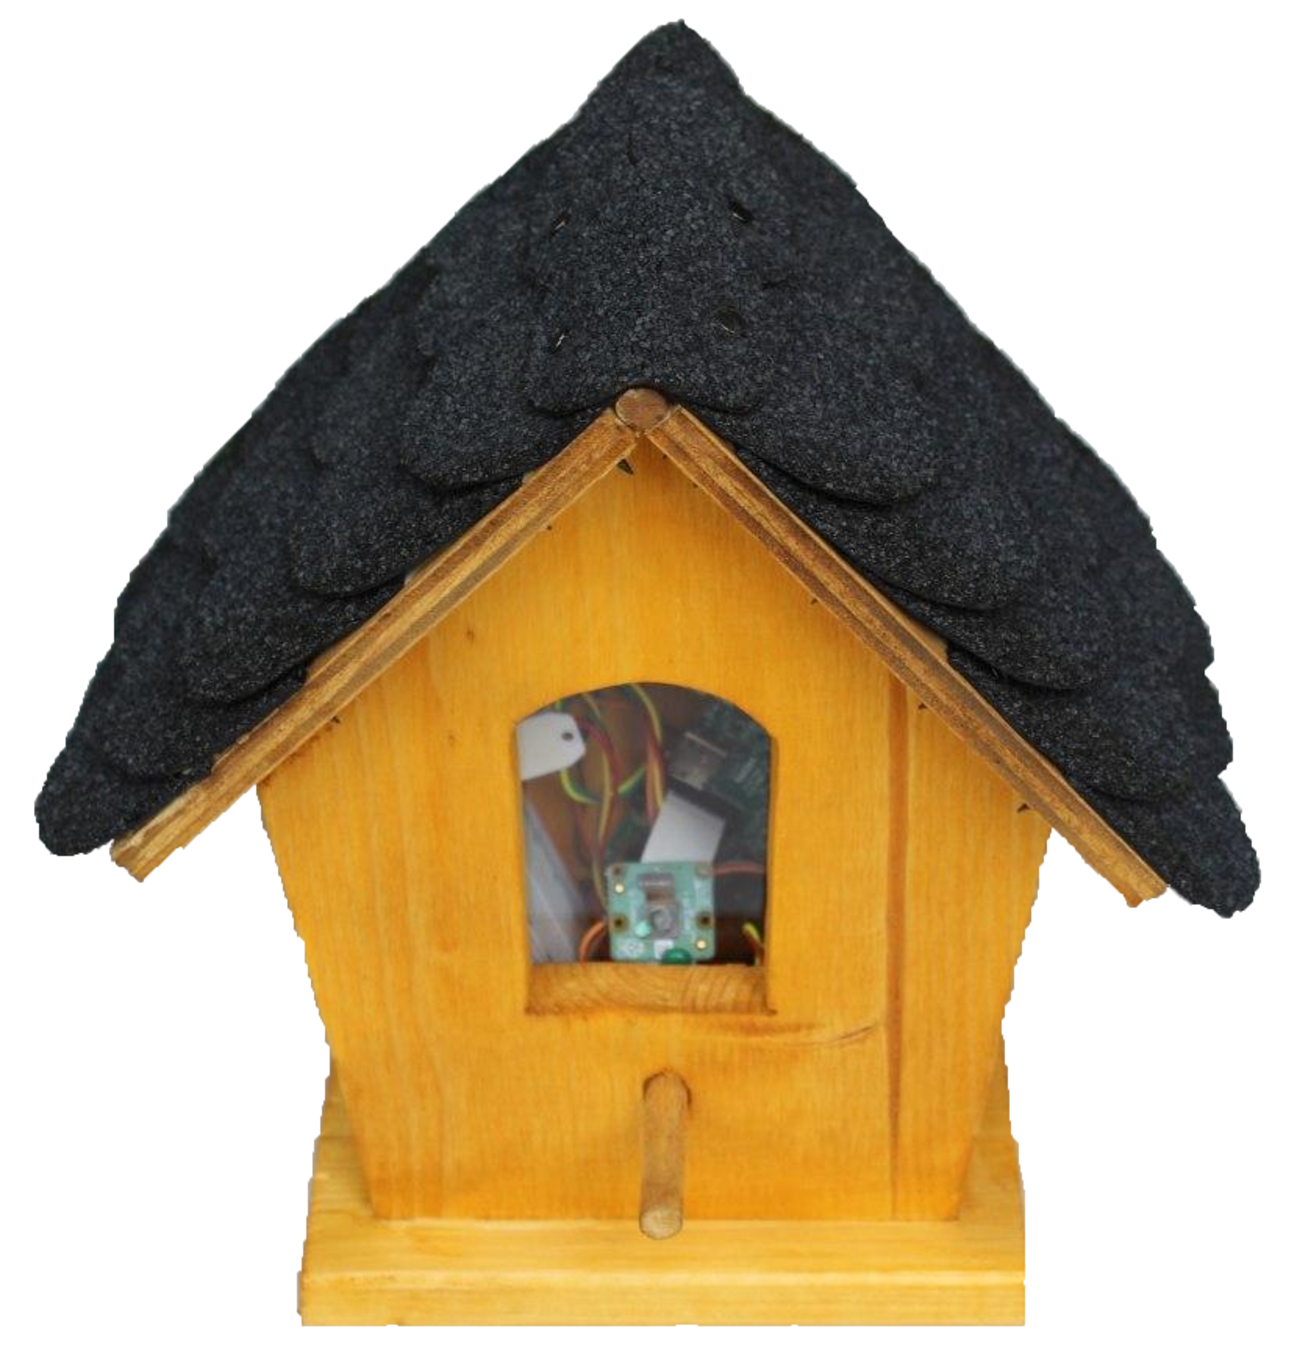
\includegraphics[width=0.4\textwidth]{./pictures/wetterstation.pdf}
		\caption{Wetterstation zur Aufnahme von Wetterdaten.}
		\label{fig:name}
		\vspace{-0.5cm}
\end{wrapfigure}
Das weatherpi Projekt entsteht im Rahmen des Physikstudiums.
Es widmet sich der Fragestellung, ob sich mit einfachen Mitteln zuverlässige
Wettervorhersagen erstellen lassen können.
Dazu werden lokale Wetterdaten mittels Sensoren, welche an einem 
Einplatinencomputer (Raspberry Pi) angeschlossen sind, erhoben.
Die aufgezeichneten Daten werden auf einen zentralen Server hochgeladen.
Ziel ist es, die lokalen Daten von mehreren Wetterstationen auszuwerten, um eine
flächendeckende Wetterprognose abzugeben. 

Zu den erhobenen Daten zählen die Temperatur, der Druck, die Luftfeuchtigkeit,
sowie ein Ausschnitt der Wolkendecke.
Inhalt dieses Papers ist die Wolkenklassifizierung, die ein Teil der
Wetteranalyse bildet.
Diese ist zur Spezifizierung der aktuellen Wetterlage notwendig.
Um Korrelationen zwischen den Attributen und der Bewölkung zu prüfen,
müssen die Daten bei bekannter Bewölkung aufgenommen werden.
Besteht eine Korrelation, so könnte in einem weiteren Schritt die Wolkendecke
als ein zusätzliches Attribut genutzt werden, um die anderen Wetterdaten genauer
vorherzusagen. 

Die erhobenen Wolkendaten sollen nach einem Training auf einem rechenstärkeren
Computer, mittels einer Live-Analyse auf dem Einplatinencomputer ausgewertet 
werden.
Die Auswertung steht unter der Prämisse schnell, genau und ressourcenschonend 
zu seien.
Dazu werden Algorithmen des maschinellen Lernenens verwendet, welche auf einen
klassifizierten Datensatz trainiert werden. 
Diese sollen bei hinreichend großer Genauigkeit die Klassenzugehörigkeit
automatisch erkennen.
Wenn das Klassenlabel bekannt ist, muss nicht mehr die gesamte Datenmenge des
Fotos zum Server geschickt werden und der Datentransfer kann reduziert werden. 
Desweiteren kann die Rechenlast auf die Rasperry Pis, welche in der Regel 
nicht ausgelastet sind, vom Server ausgelagert werden. 

Dazu werden zwei Modelle evaluiert, welche auf den charakteristischen
Eigenschaften des Wolkenspektrums trainiert werden. 
Diese sind einerseits die Formen und andererseits das Farbspektrum der Wolken.
Aus dem aufgenommenen Foto wird ein diskretes Farbspektrum erstellt, welches 
mit einem Random Forest ausgewertet werden kann.
Dabei bietet der Random Forest ein hohen Schutz gegen Übertraining.
Mittels eines Convolutional Neuronal Network (CNN) besteht die Möglichkeit, auf
dem Farbspektrum der Wolken sowie deren Formen zu trainieren. 
Die erhöhte Informationsdichte, mit der das CNN trainiert werden kann, 
lässt bei einem ausreichend generalisierten Training auf einen leistungs 
Schub gegenüber dem Random Forest schließen.

% Werden die Wolken entsprechend richtig klassifiziert laesst sich in weiteren
% Schritten welche nicht Teil dieses Papers sind aus der Folge der Wolken z.B
% der Niederschlag berechnen. 
% Desweiteren kann die entwicklung der Temperatur aufgrund der Waermespeicherung
% und Isolierug von Wolken verbessert werden.


\section{Datensatz}
\label{sec:02_Datensatz}

Der Datensatz wurde mittels einer PiCamera in einem Zeitraum von 3 Wochen
aufgenommen. 
Die Größe des Datensatzes ist beliebig erweiterbar, aber wurde aufgrund der
zeitlichen Einschränkung zur Evaluation auf \num{4000} Fotos beschränkt. 

\begin{wrapfigure}{l}{0.35\textwidth}
		\centering
		\vspace{-0.5cm}
		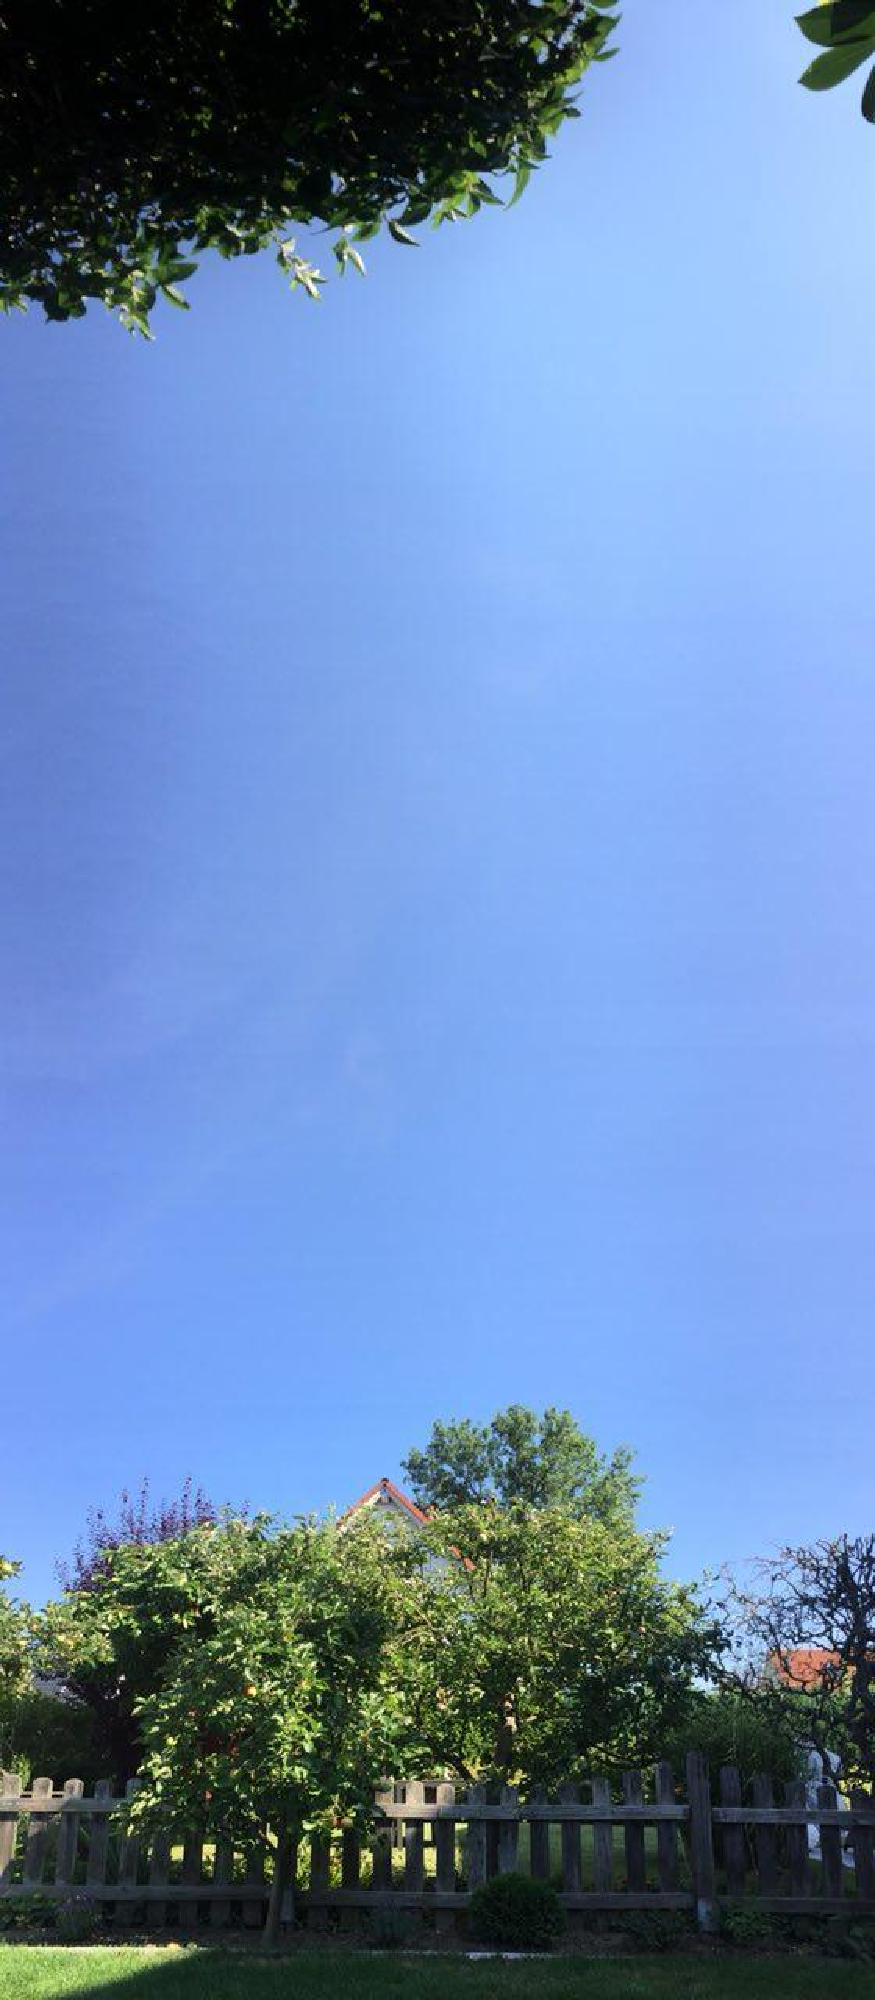
\includegraphics[width=0.3\textwidth]{./build/station_winkel.pdf}
		\caption{Wolkenausschnitt in Abhängigkeit des Observationswinkels.}
		\label{fig:theta}
		\vspace{-0.5cm}
\end{wrapfigure}
Desweiteren spielt die Zeit in der die Daten aufgenommen werden eine 
wesentliche Rolle.
In Abhängigkeit mit der Jahreszeiten ändern sich die relativen Häufigkeit, in 
der die verschiedene Wolkentypen aufgenommen werden können und somit in dem 
Datensatz repräsentiert sind. 
So sind zum Beispiel momentan (\today) Schönwetterwolken viel häufiger
vertreten, als die von Regenwetter. 
Zu den elf Wolkenklassen, die auch die Klasse \textit{keine Wolken} einschließt, 
zählt ebenso eine \textit{schlechtes Foto} Klasse. 
Aufgrund von zufälligen als auch zeitlichen Ereignissen werden Fotos produziert
die nicht Klassifiziert werden können.
Dies ist beispielsweise der Fall, wenn eine Person das Sichtfeld verdeckt oder 
aufgrund der fehlenden Belichtung bei Nacht die Wolkendecke nicht erkannt wird.

Die Wolkenfotos wurden an zwei voneinander unabhängigen Orten aufgenommen, wobei
Charakteristiken der Aufnahmeorte auf den Bildern zu erkennen sein können.
Desweiteren stellte sich bei der Aufnahme des Datensatzes heraus, dass eine
Ausrichtung der Kamera der Wetterstation nach Norden sinnvoll ist.
Dadurch lässt sich der Kamerasensor schonen, indem ein übermäßiges Ausleuchten
 des Bildes durch die Sonne verhindert wird.

Durch die Ausrichtung der Kamera zum Horizont kann, wie in Abbildung
 \ref{fig:theta} dargestellt, die Größe der observierten Wolkenfläche 
eingestellt werden.
Dadurch, dass die Wolken bei großen Aufnahmewinkeln $\omega$ viel näher als bei
kleinen $\omega$ sind, kann bei gleichbleibender Raumwinkelauflösung $\Omega$
nur ein viel kleinerer Teil der Wolkendecke observiert werden.
Bei diesen Ausschnitten stellt es sich als schwierig heraus, sie der richtigen
Klasse zuzuordnen, da der Ausschnitt meist mehreren Klassen zuzuordnen ist. 

\begin{wrapfigure}{r}{0.35\textwidth}
		\vspace{-1.4cm}
		\centering
		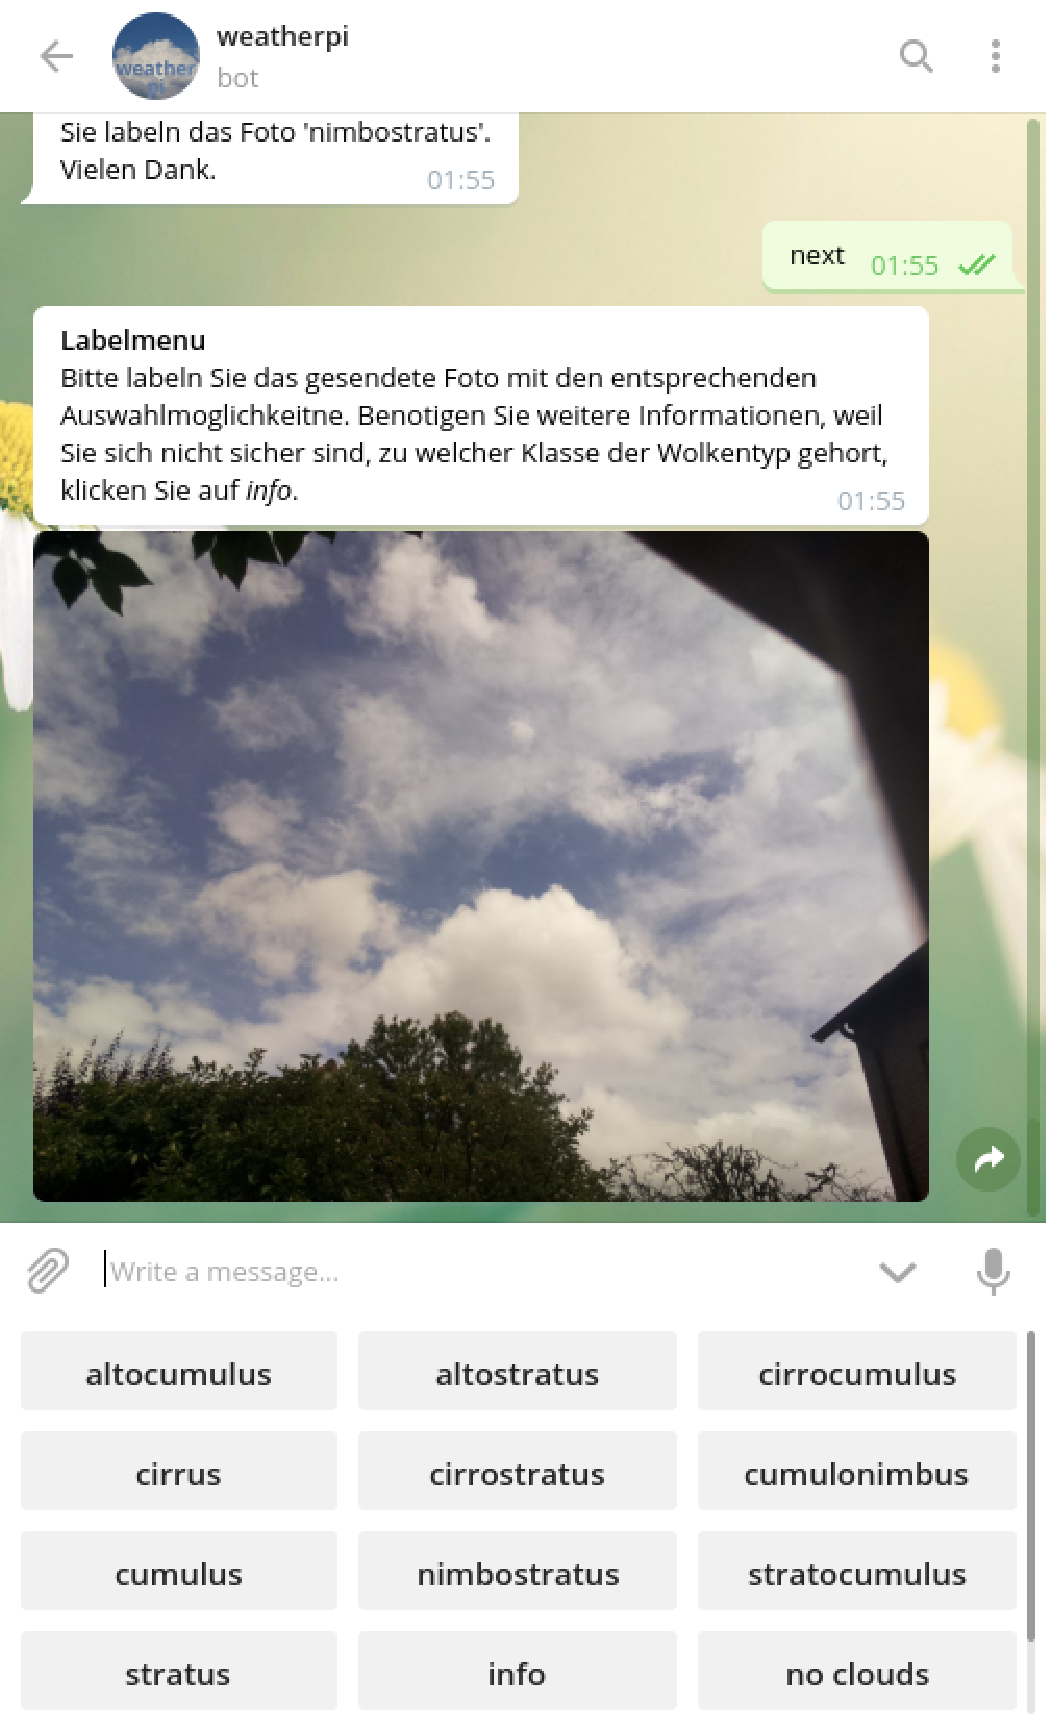
\includegraphics[width=0.35\textwidth]{pictures/telegram.pdf}
		\caption{\href{https://telegram.me/weatherpi_bot}{\texttt{TelegramBot}} zum Labeln der Wolkenfotos.}
		\label{fig:}
		\vspace{-1.0cm}
\end{wrapfigure}
Die aufgenommenen Daten besitzen a priori kein Label und sind auch nicht immer
eindeutig einer Klasse zuzuordnen.
Die Wolkenfotos wurden mittels eines eigen dafür programmierten
\href{https://telegram.me/weatherpi_bot}{\texttt{TelegramBot}} in
die in Abbildung~\ref{fig:classes} aufgeführten Kategorien eingeteilt.
Mit Hilfe von freiwilligen Labelern wurde jedes Foto des Datensatzes drei mal
gelabelt und anschließend per Mehrheitsentscheidung der Zielklasse 
zugeteilt.
Der Arbeitsaufwand wurde mit ca $\num{4000} \, \text{Bilder} \cdot \SI{1}{\hertz}$
abgeschätzt.
Aufgrund von Aussetzern des Bots und der Ladezeiten der Bilder konnte die Rate
auch nach einer Einarbeitungszeit nicht erreicht werden und die pro Bild benötigte Zeit entsprach schätzungsweise
\SI{15}{\second}.
Bei der Evaluation der Modelle stellte sich heraus, dass bei paralleler Nutzung
eine interne Klassenvariable überschrieben wurde, sodass ein Großteil der
Klassifizierten Daten einer falschen finalen Klasse zugeordnet wurden. 
Final steht ein Datensatz von \num{4000} Bildern welche in 10 Wolkenklassen und
einer Klasse mit schlechten Fotos aufgeteilt sind. Die Bilder besitzen eine Dimension 
von \texttt{(1024x768x3)} und liegen im \texttt{JPG}-Format vor.
Sie stehen unter der MIT Lizens und soll allen interessierten 
Datenanalysten zur Verfügung stehen.

\begin{figure}[h]
		\centering
		\begin{subfigure}[b]{0.31\textwidth}
		\begin{center}
				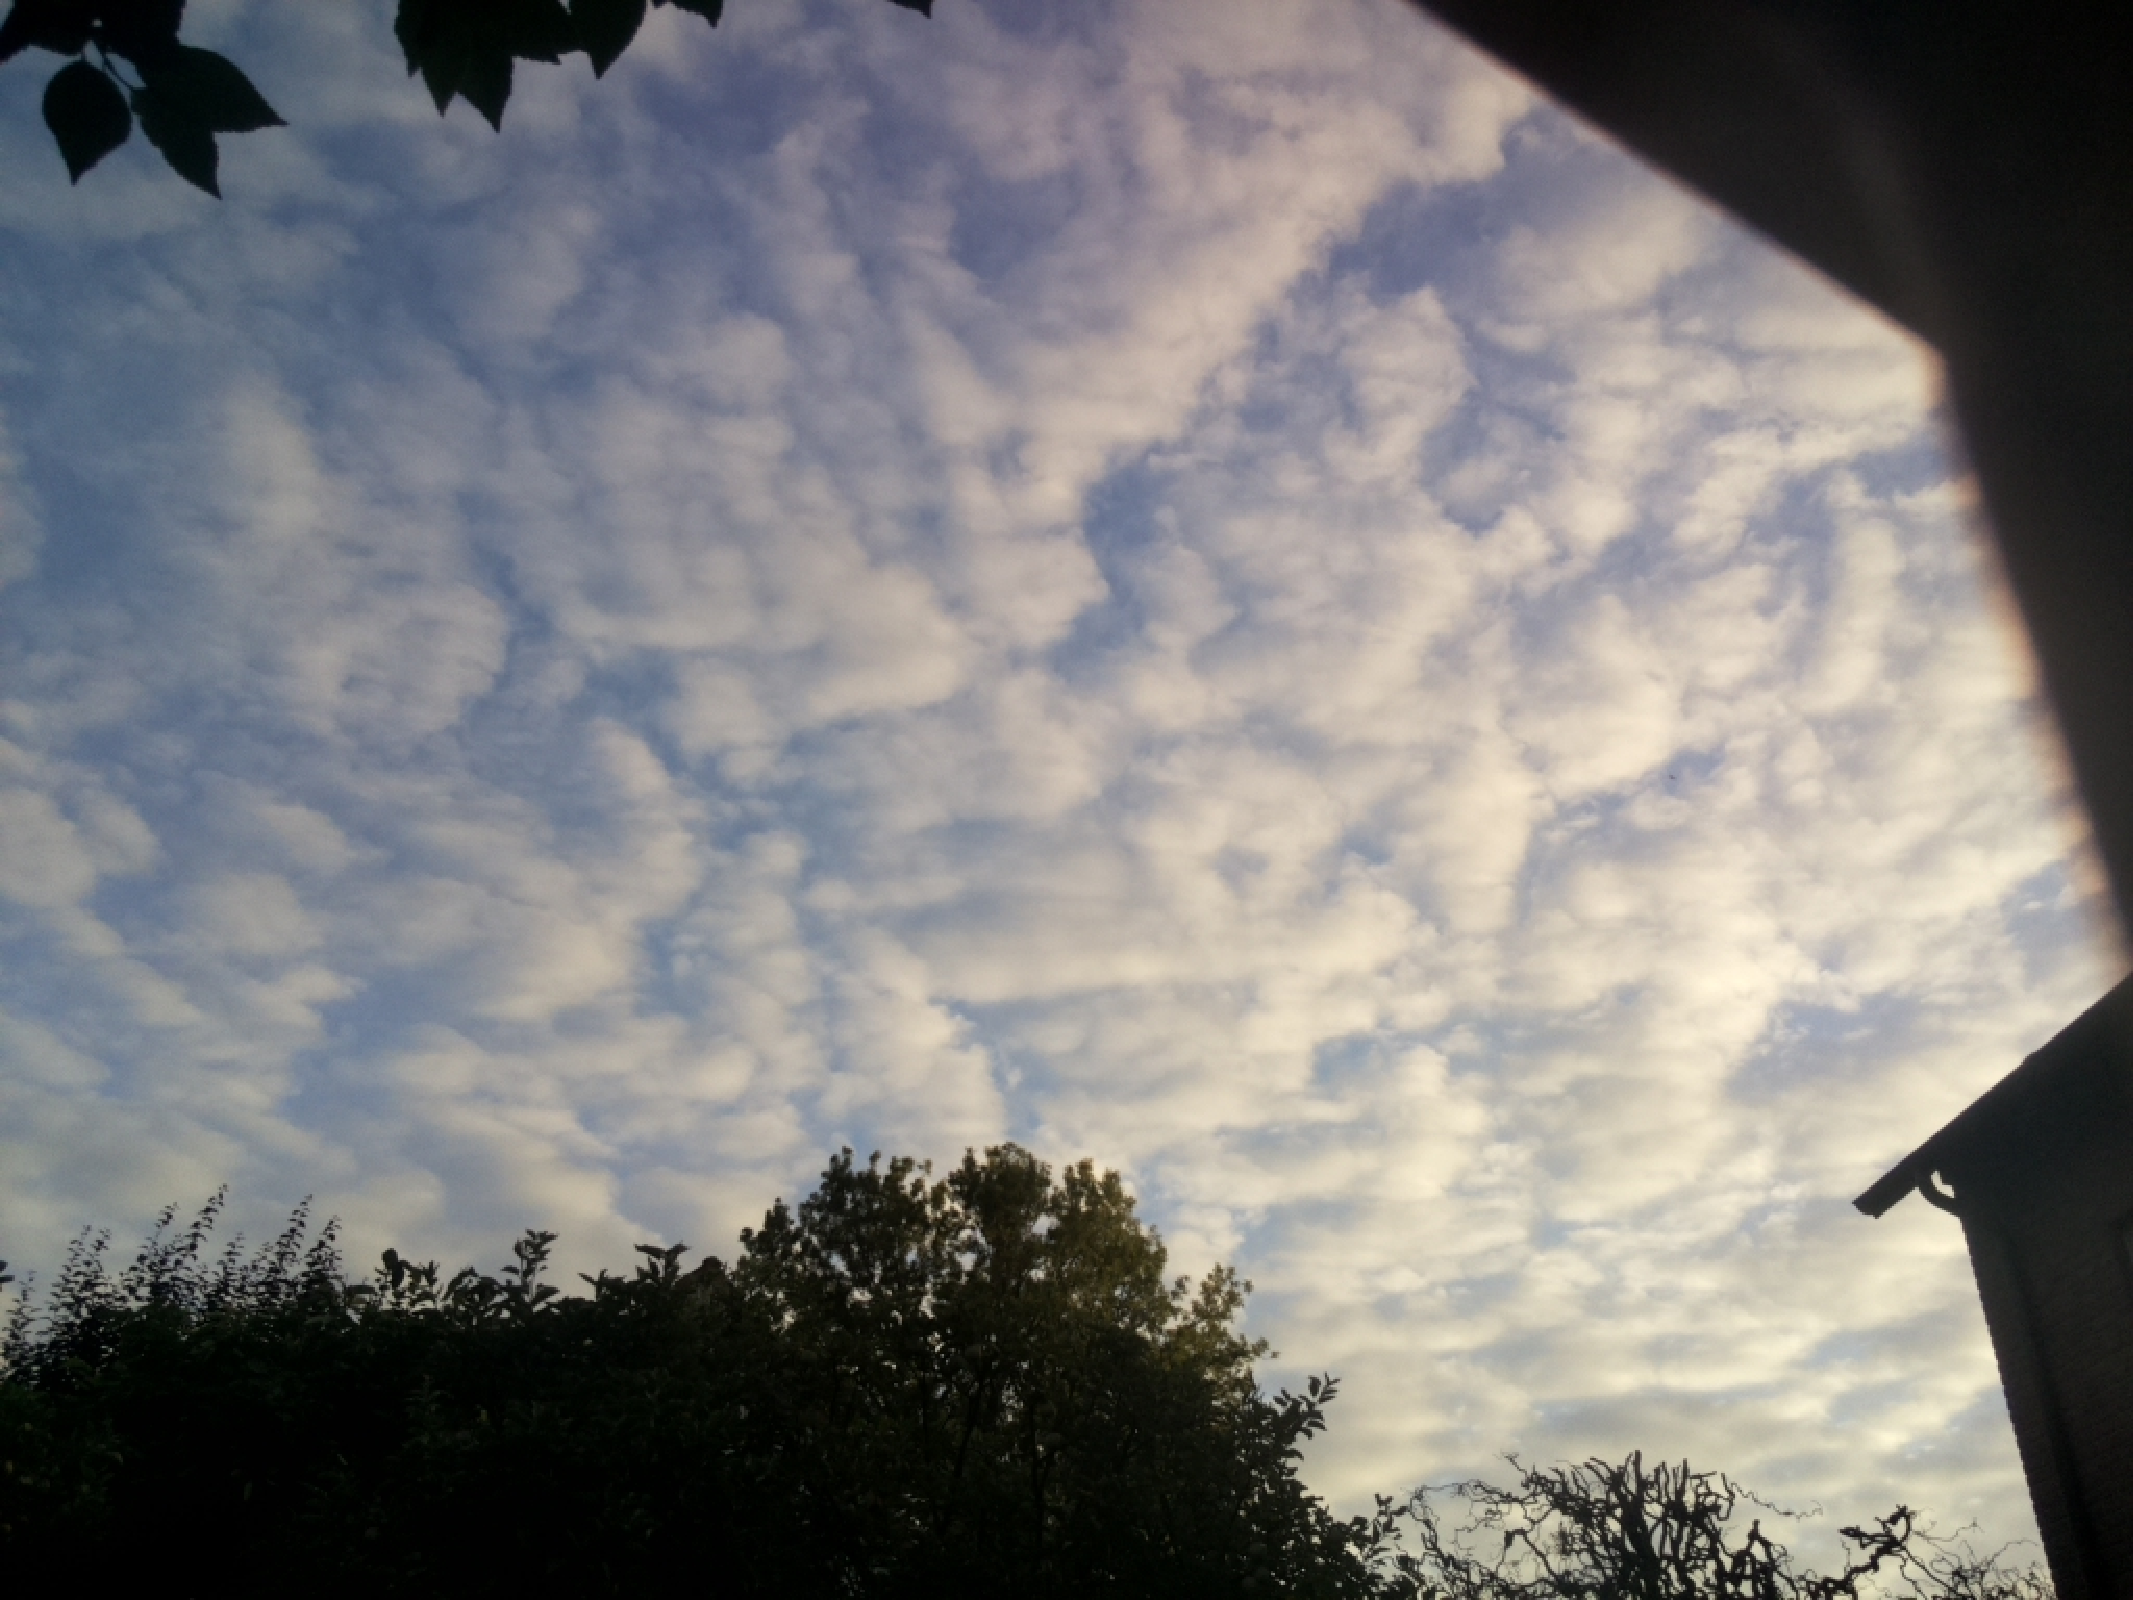
\includegraphics[width=\textwidth]{./pictures/cloudtypes/altocumulus.pdf}
		\end{center}
		\caption{Altocumulus}
		\label{fig:altostratus}
		\end{subfigure}
		\begin{subfigure}[b]{0.31\textwidth}
		\begin{center}
				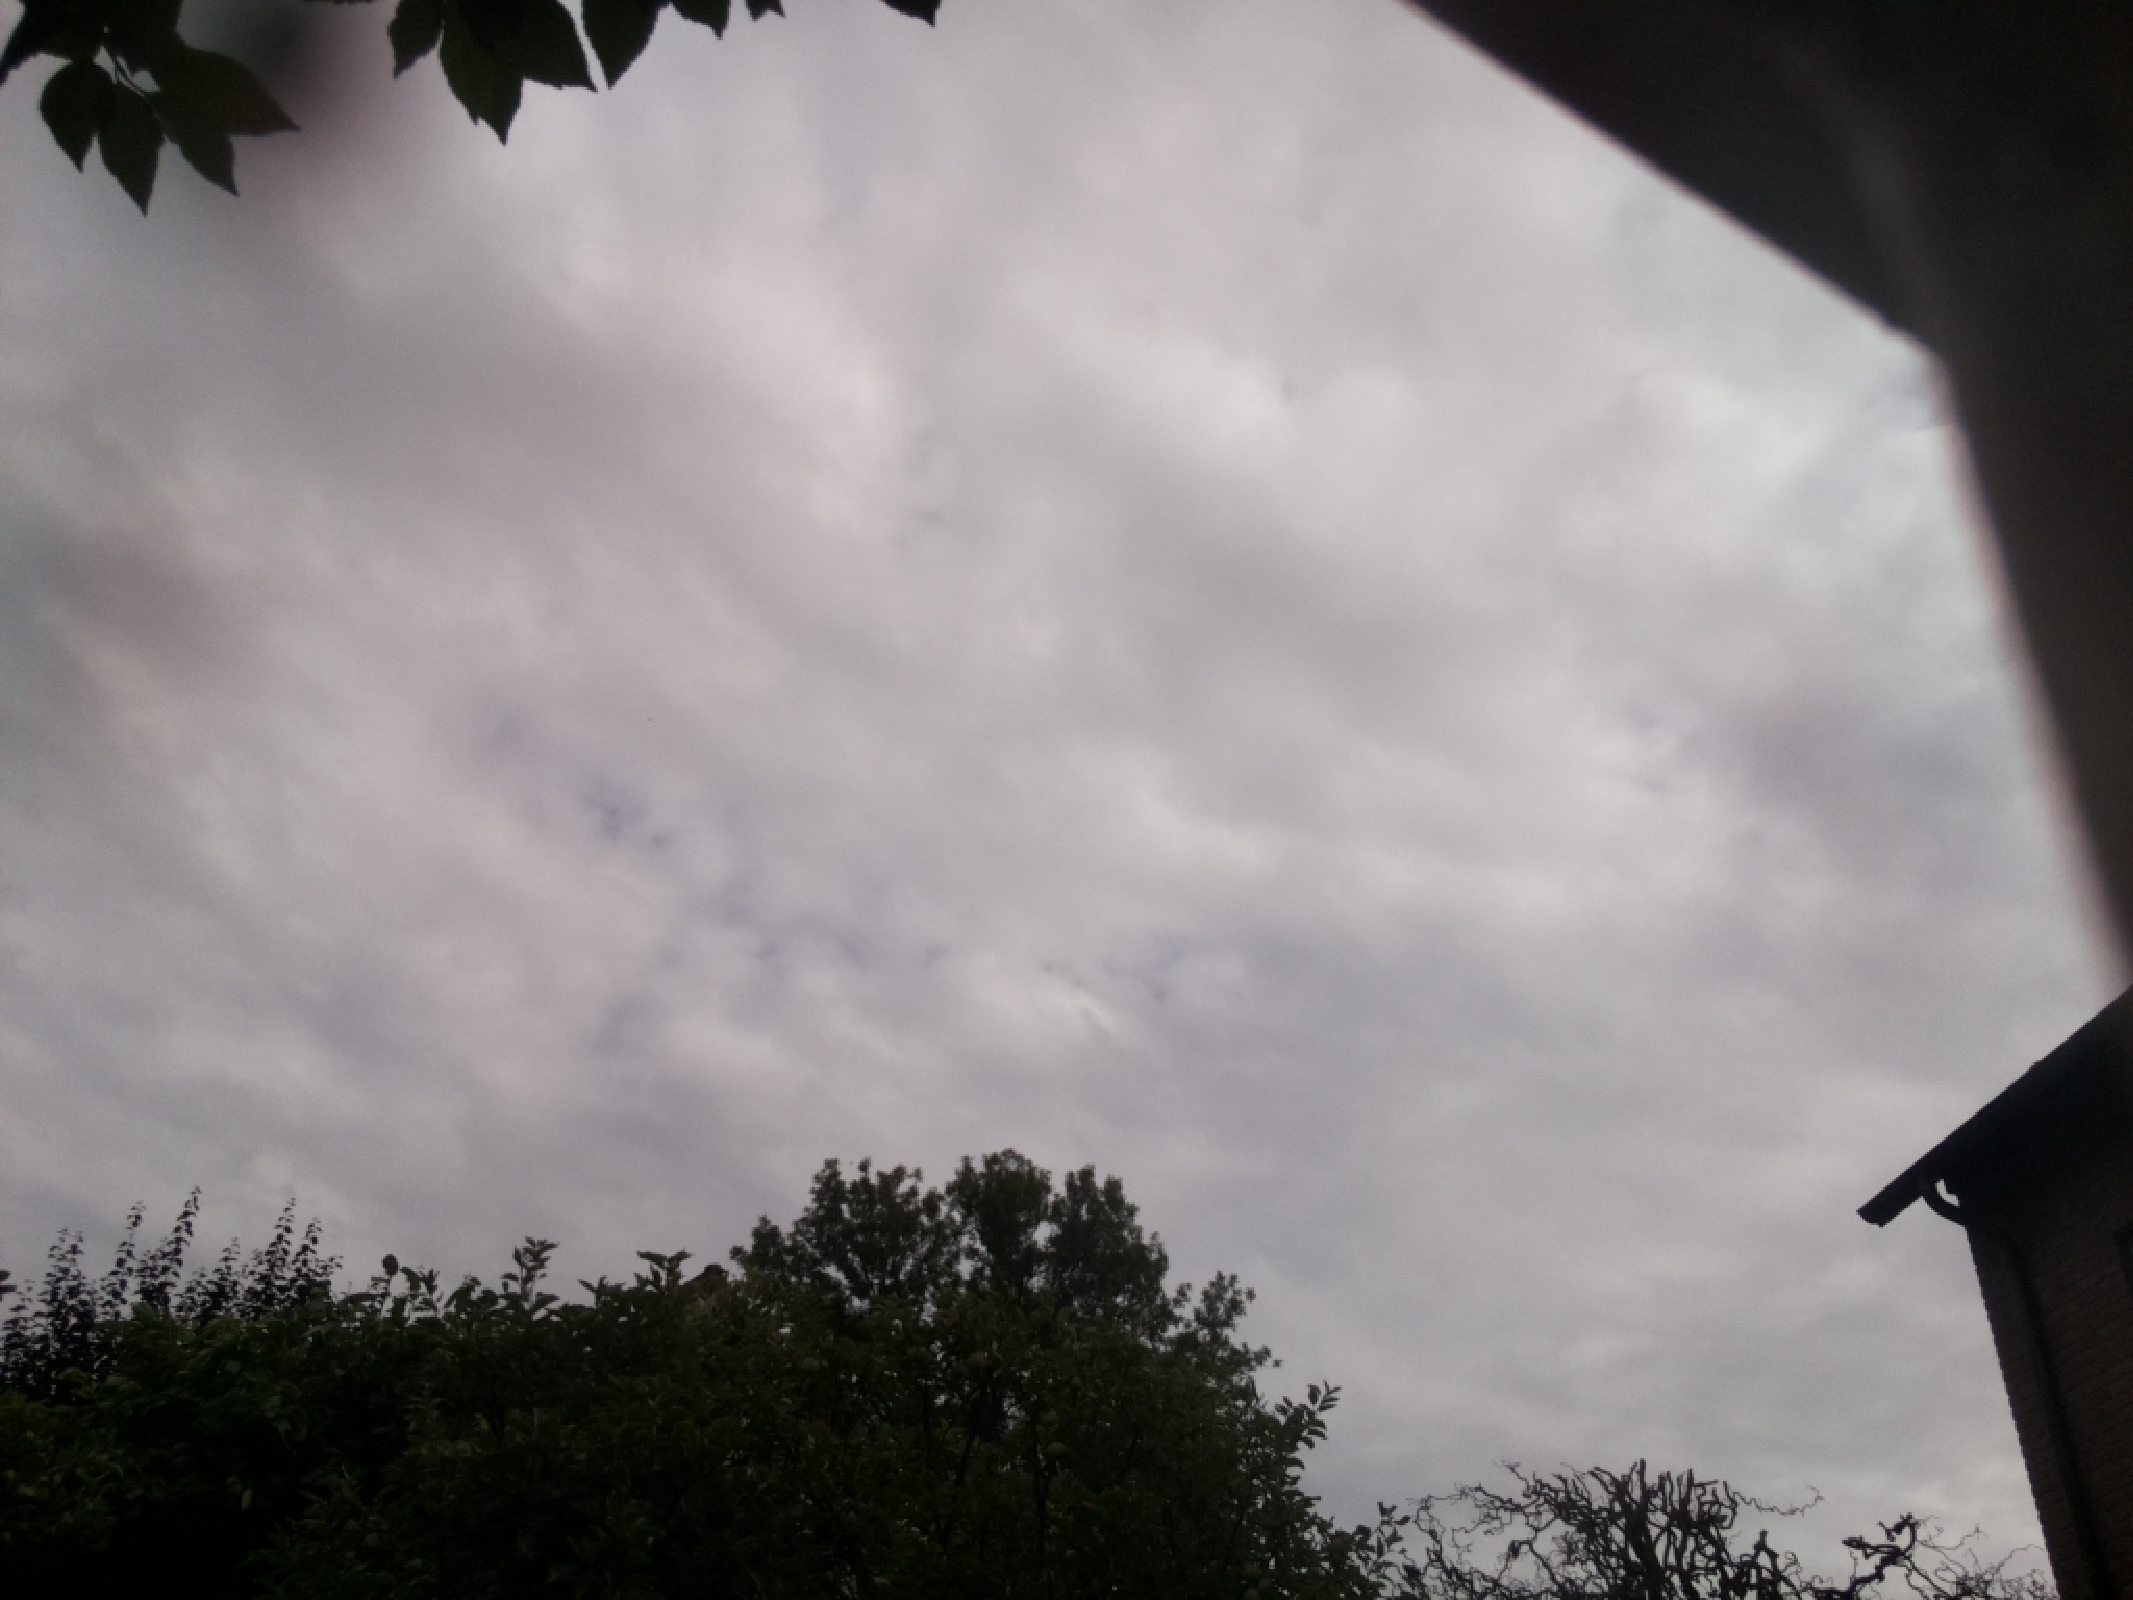
\includegraphics[width=\textwidth]{./pictures/cloudtypes/altostratus.pdf}
		\end{center}
		\caption{Altostratus}
		\label{fig:altocumulus}
		\end{subfigure}
		\begin{subfigure}[b]{0.31\textwidth}
		\begin{center}
				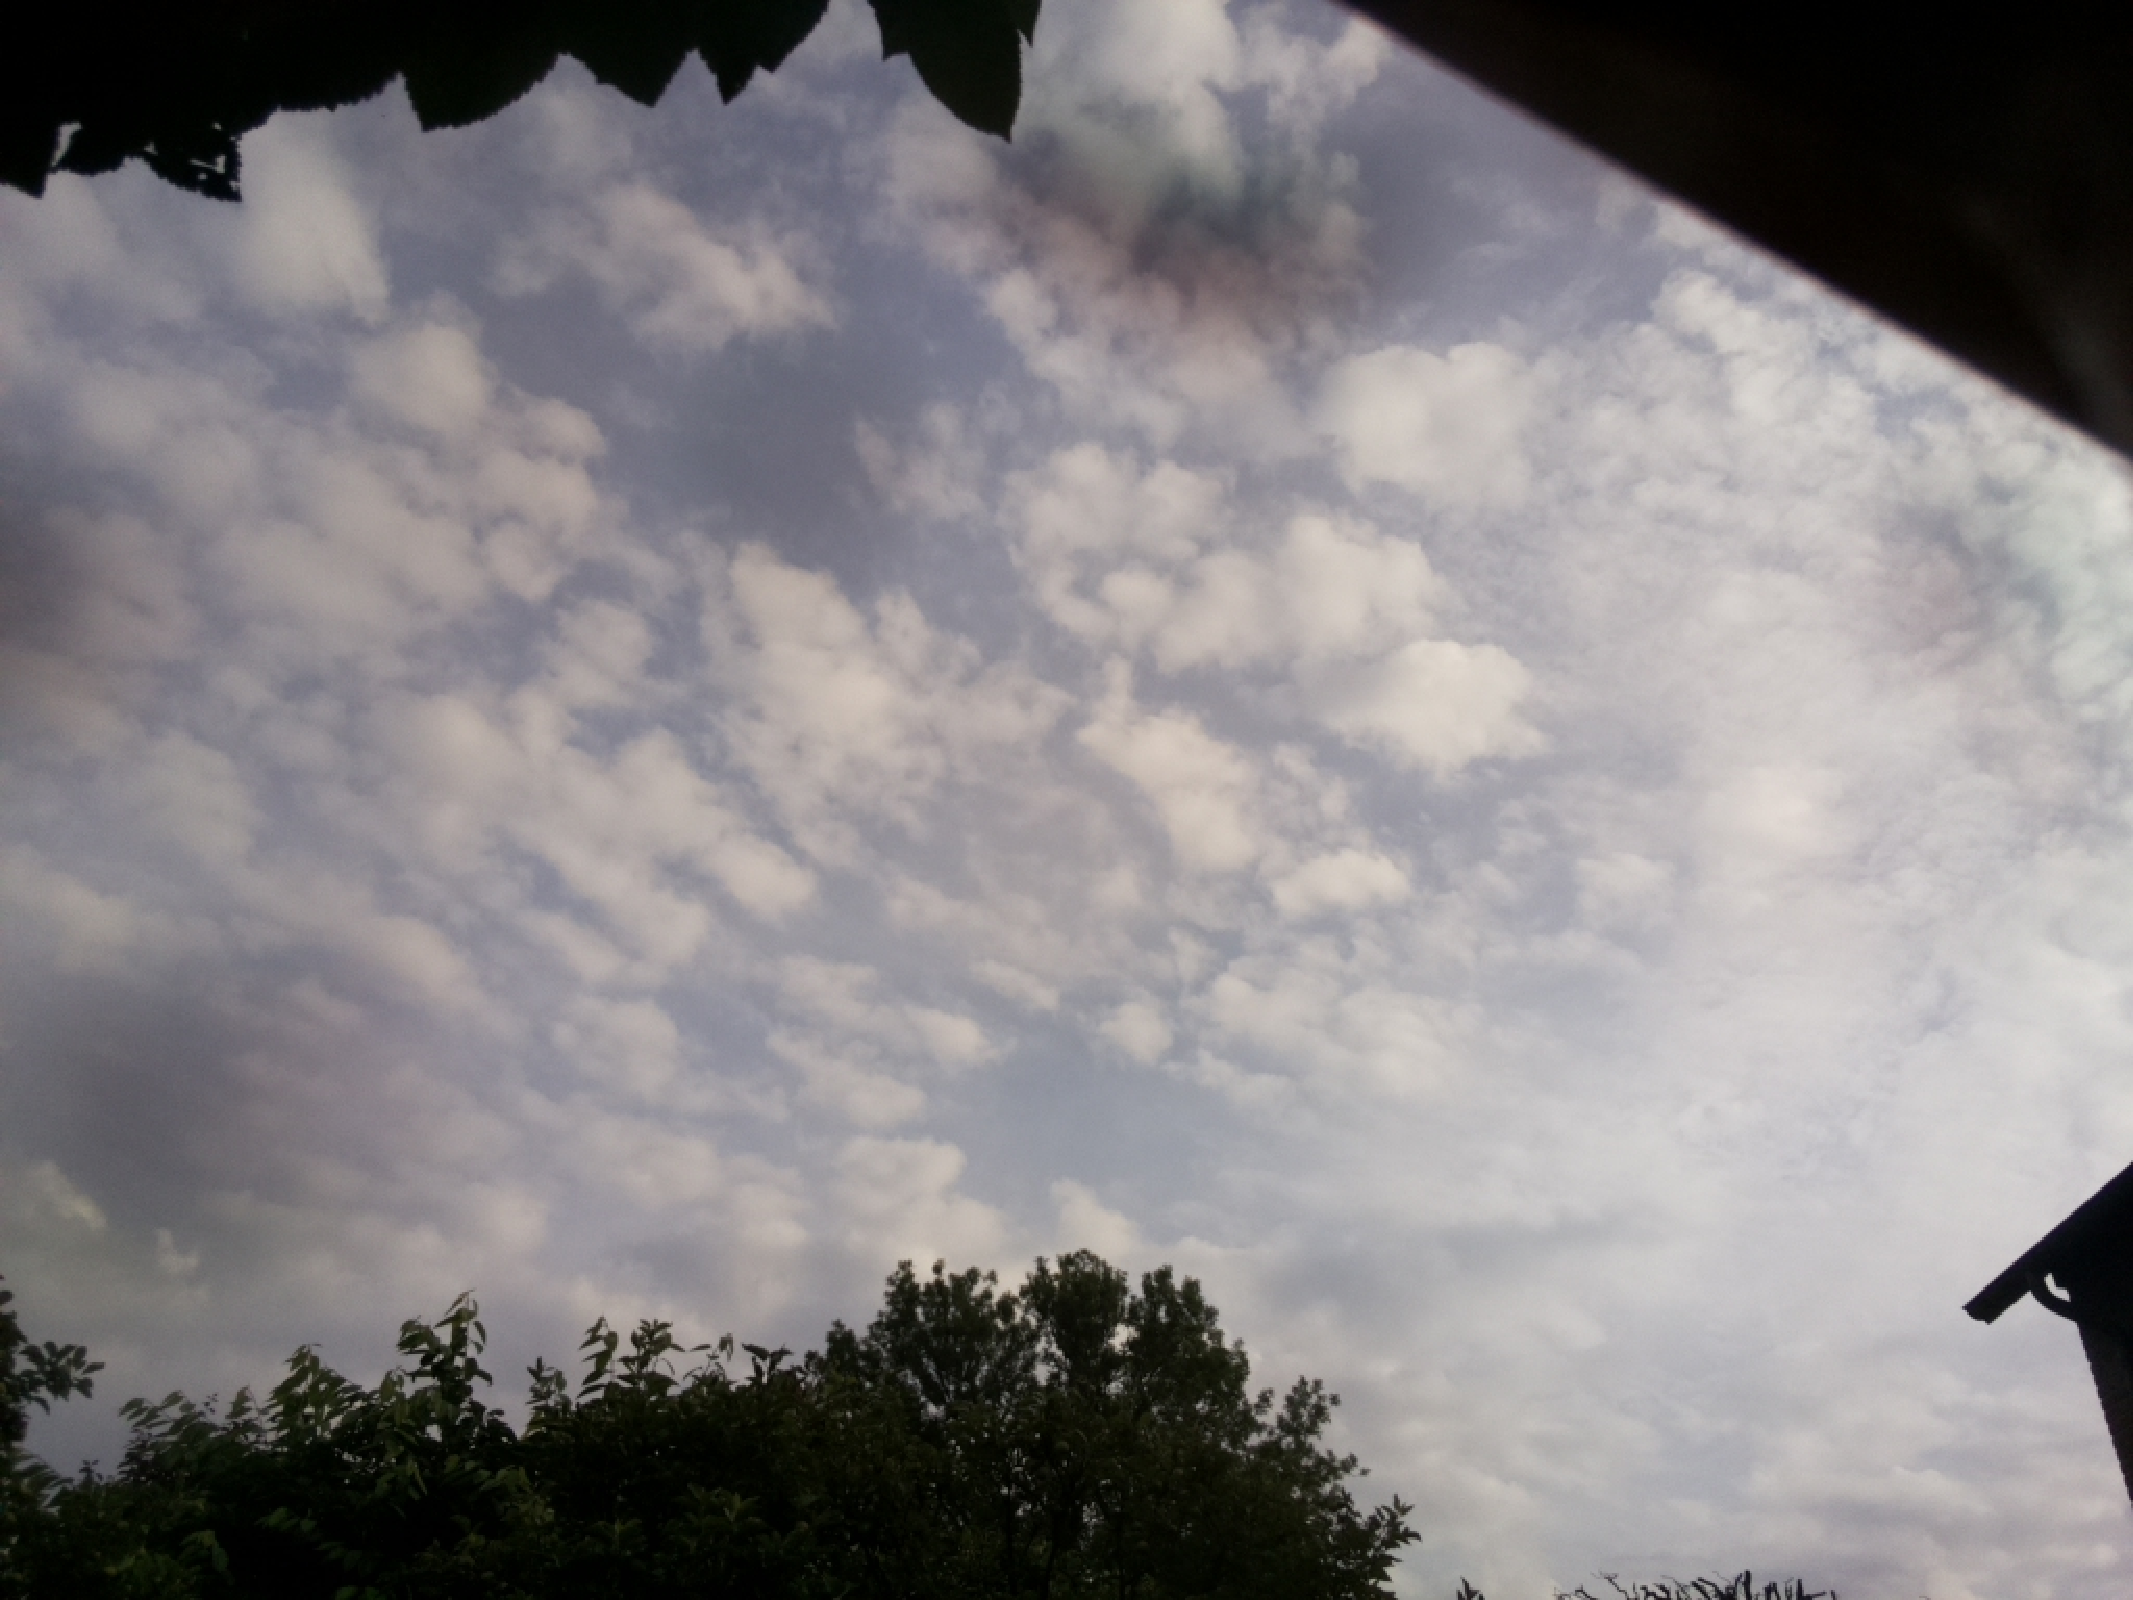
\includegraphics[width=\textwidth]{./pictures/cloudtypes/cirrocumulus.pdf}
		\end{center}
		\caption{Cirrocumulus}
		\label{fig:cirrocumulus}
		\end{subfigure}
		\begin{subfigure}[b]{0.31\textwidth}
		\begin{center}
				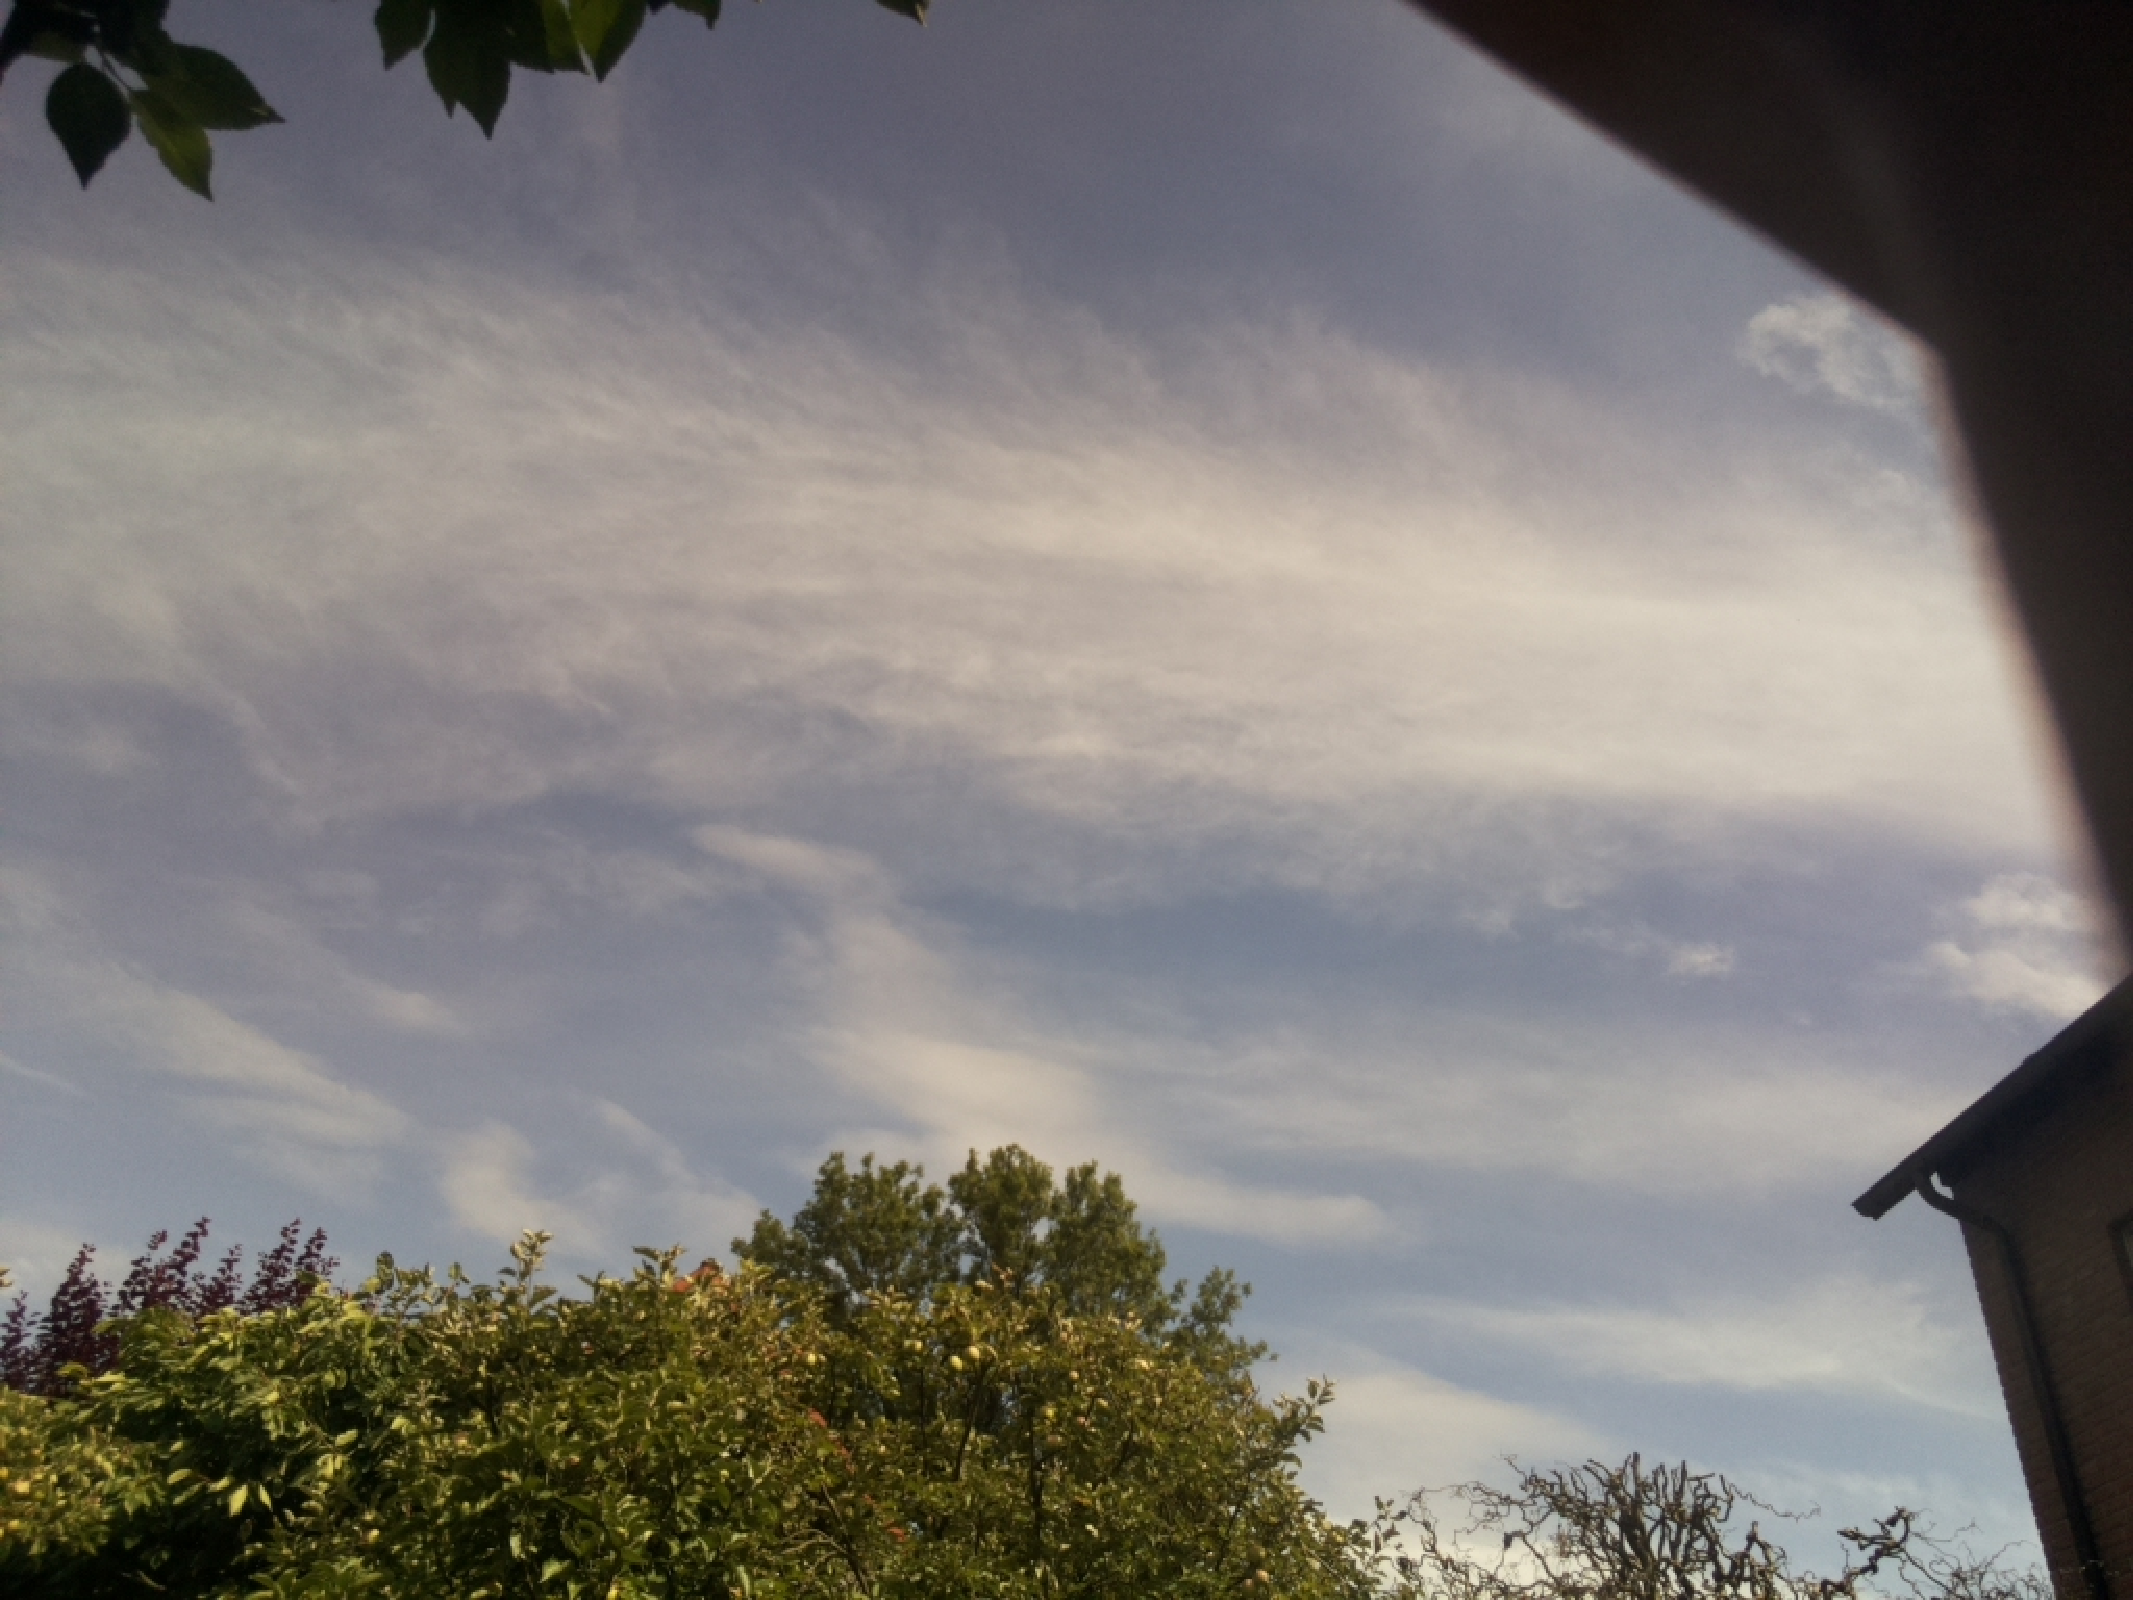
\includegraphics[width=\textwidth]{./pictures/cloudtypes/cirrostratus.pdf}
		\end{center}
		\caption{Cirrostratus}
		\label{fig:cirrostratus}
		\end{subfigure}
		\begin{subfigure}[b]{0.31\textwidth}
		\begin{center}
				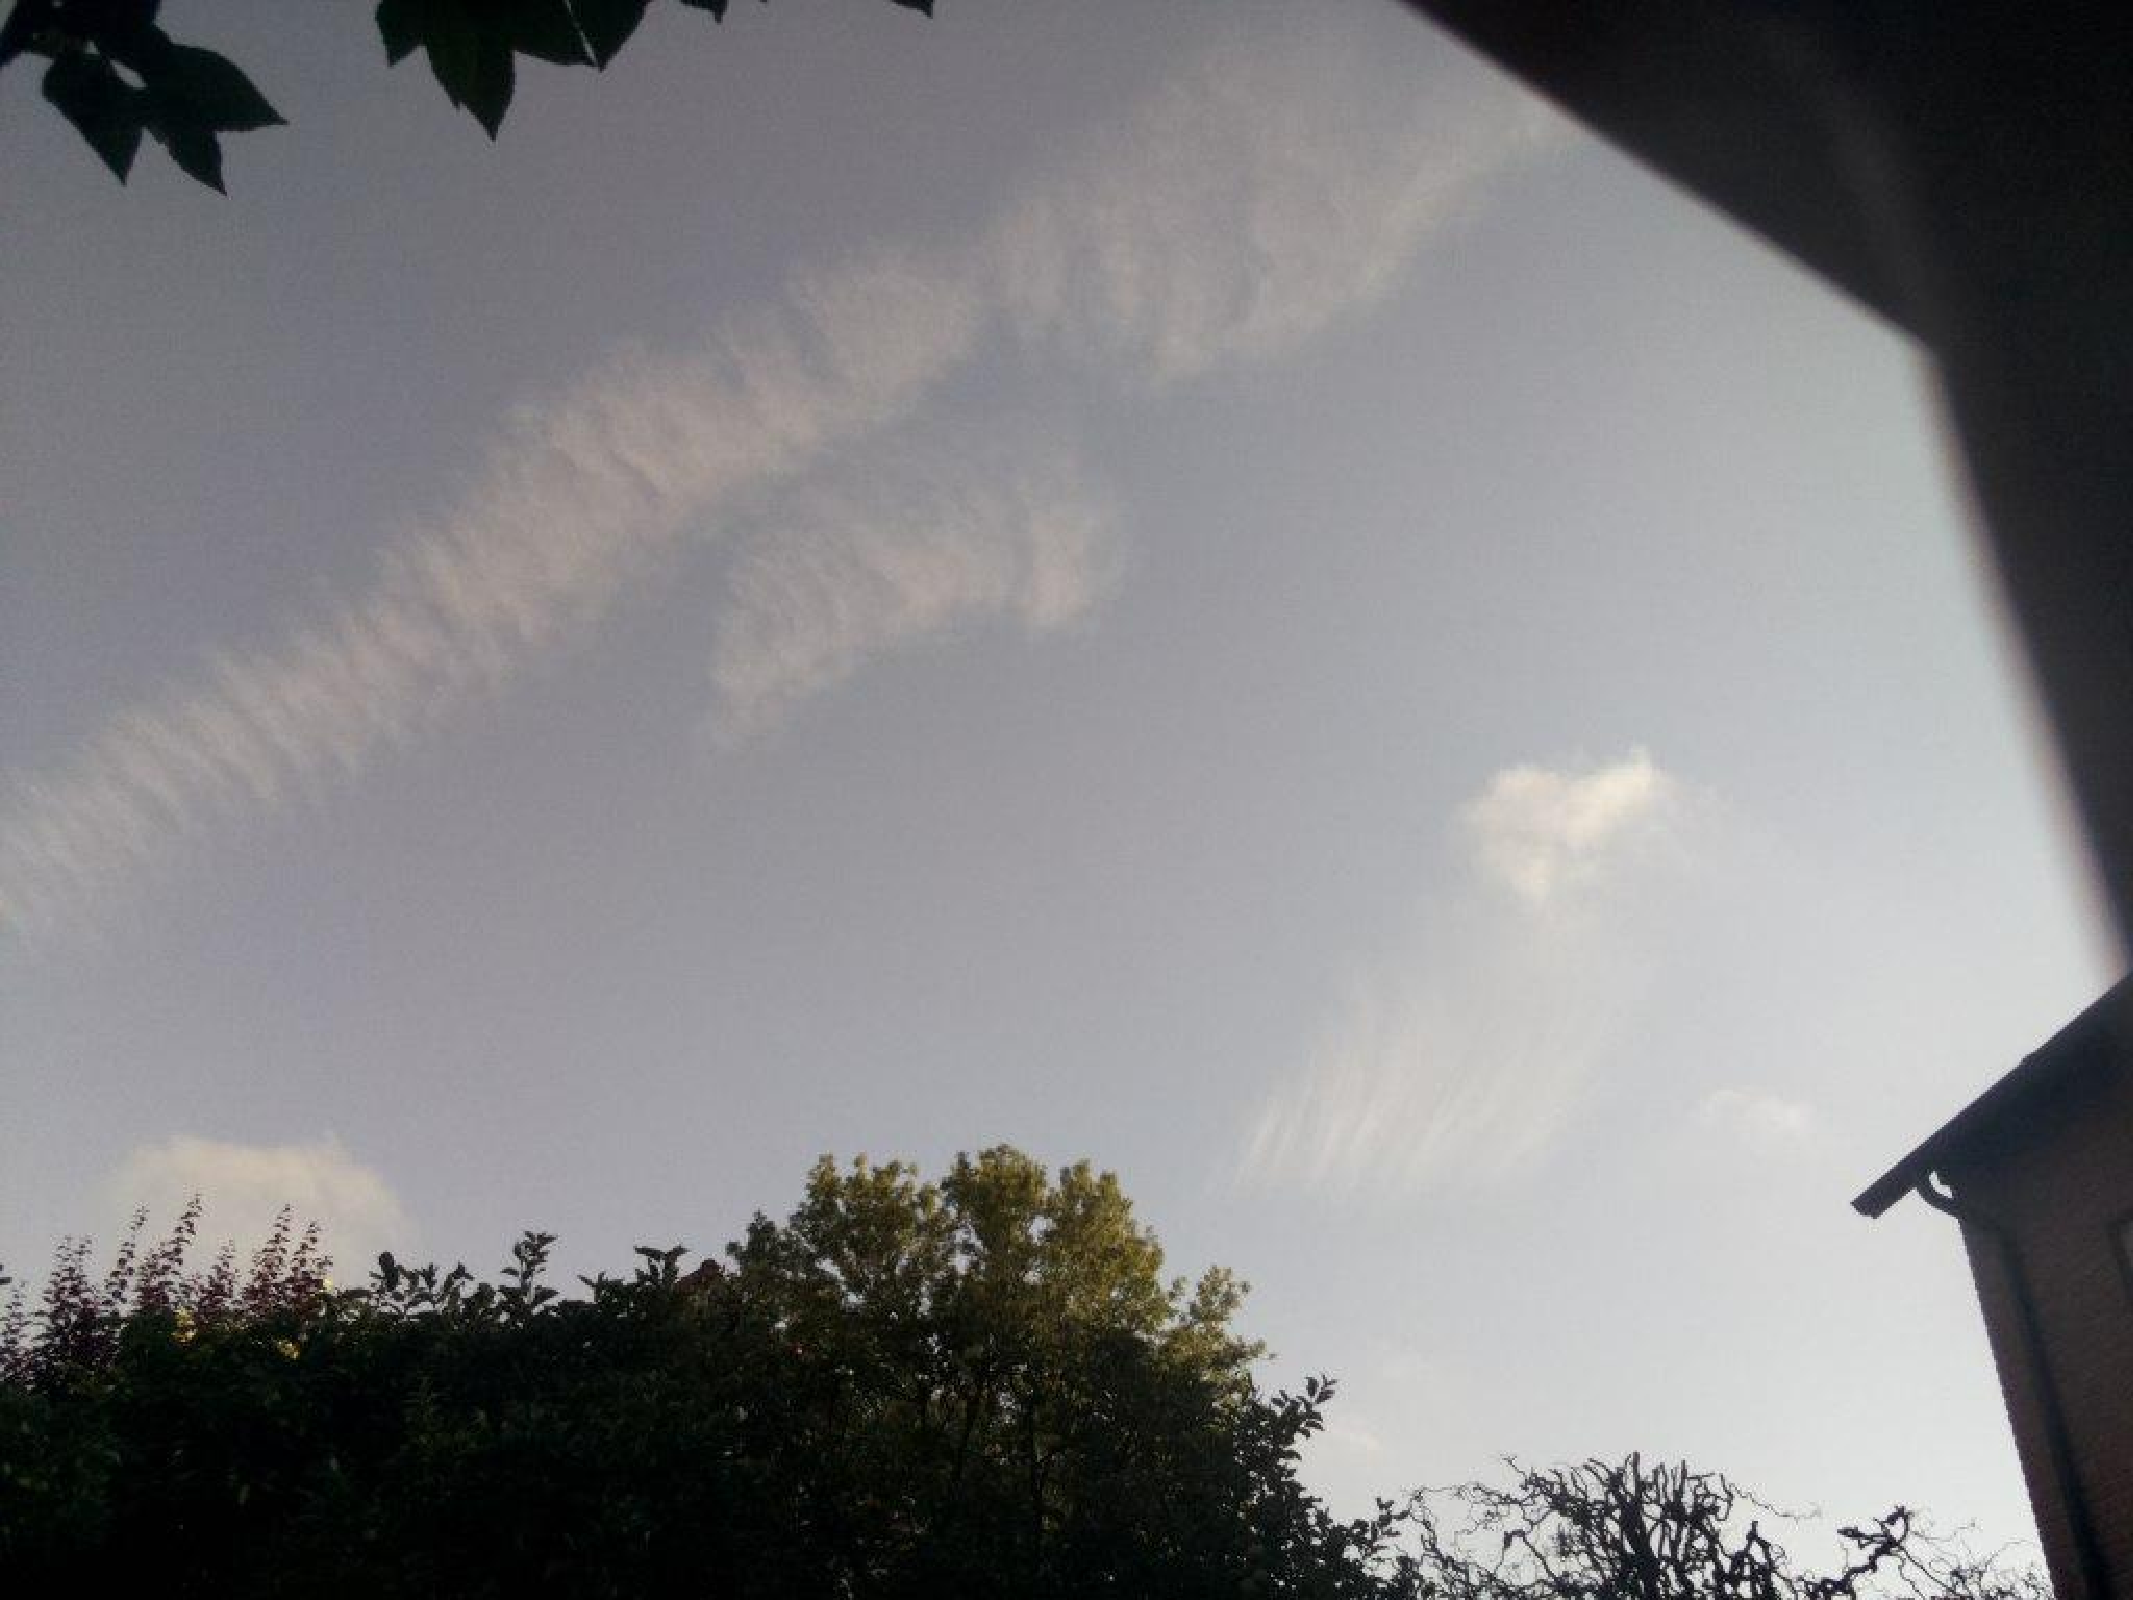
\includegraphics[width=\textwidth]{./pictures/cloudtypes/cirrus.pdf}
		\end{center}
		\caption{Cirrus}
		\label{fig:cirrus}
		\end{subfigure}
		\begin{subfigure}[b]{0.31\textwidth}
		\begin{center}
				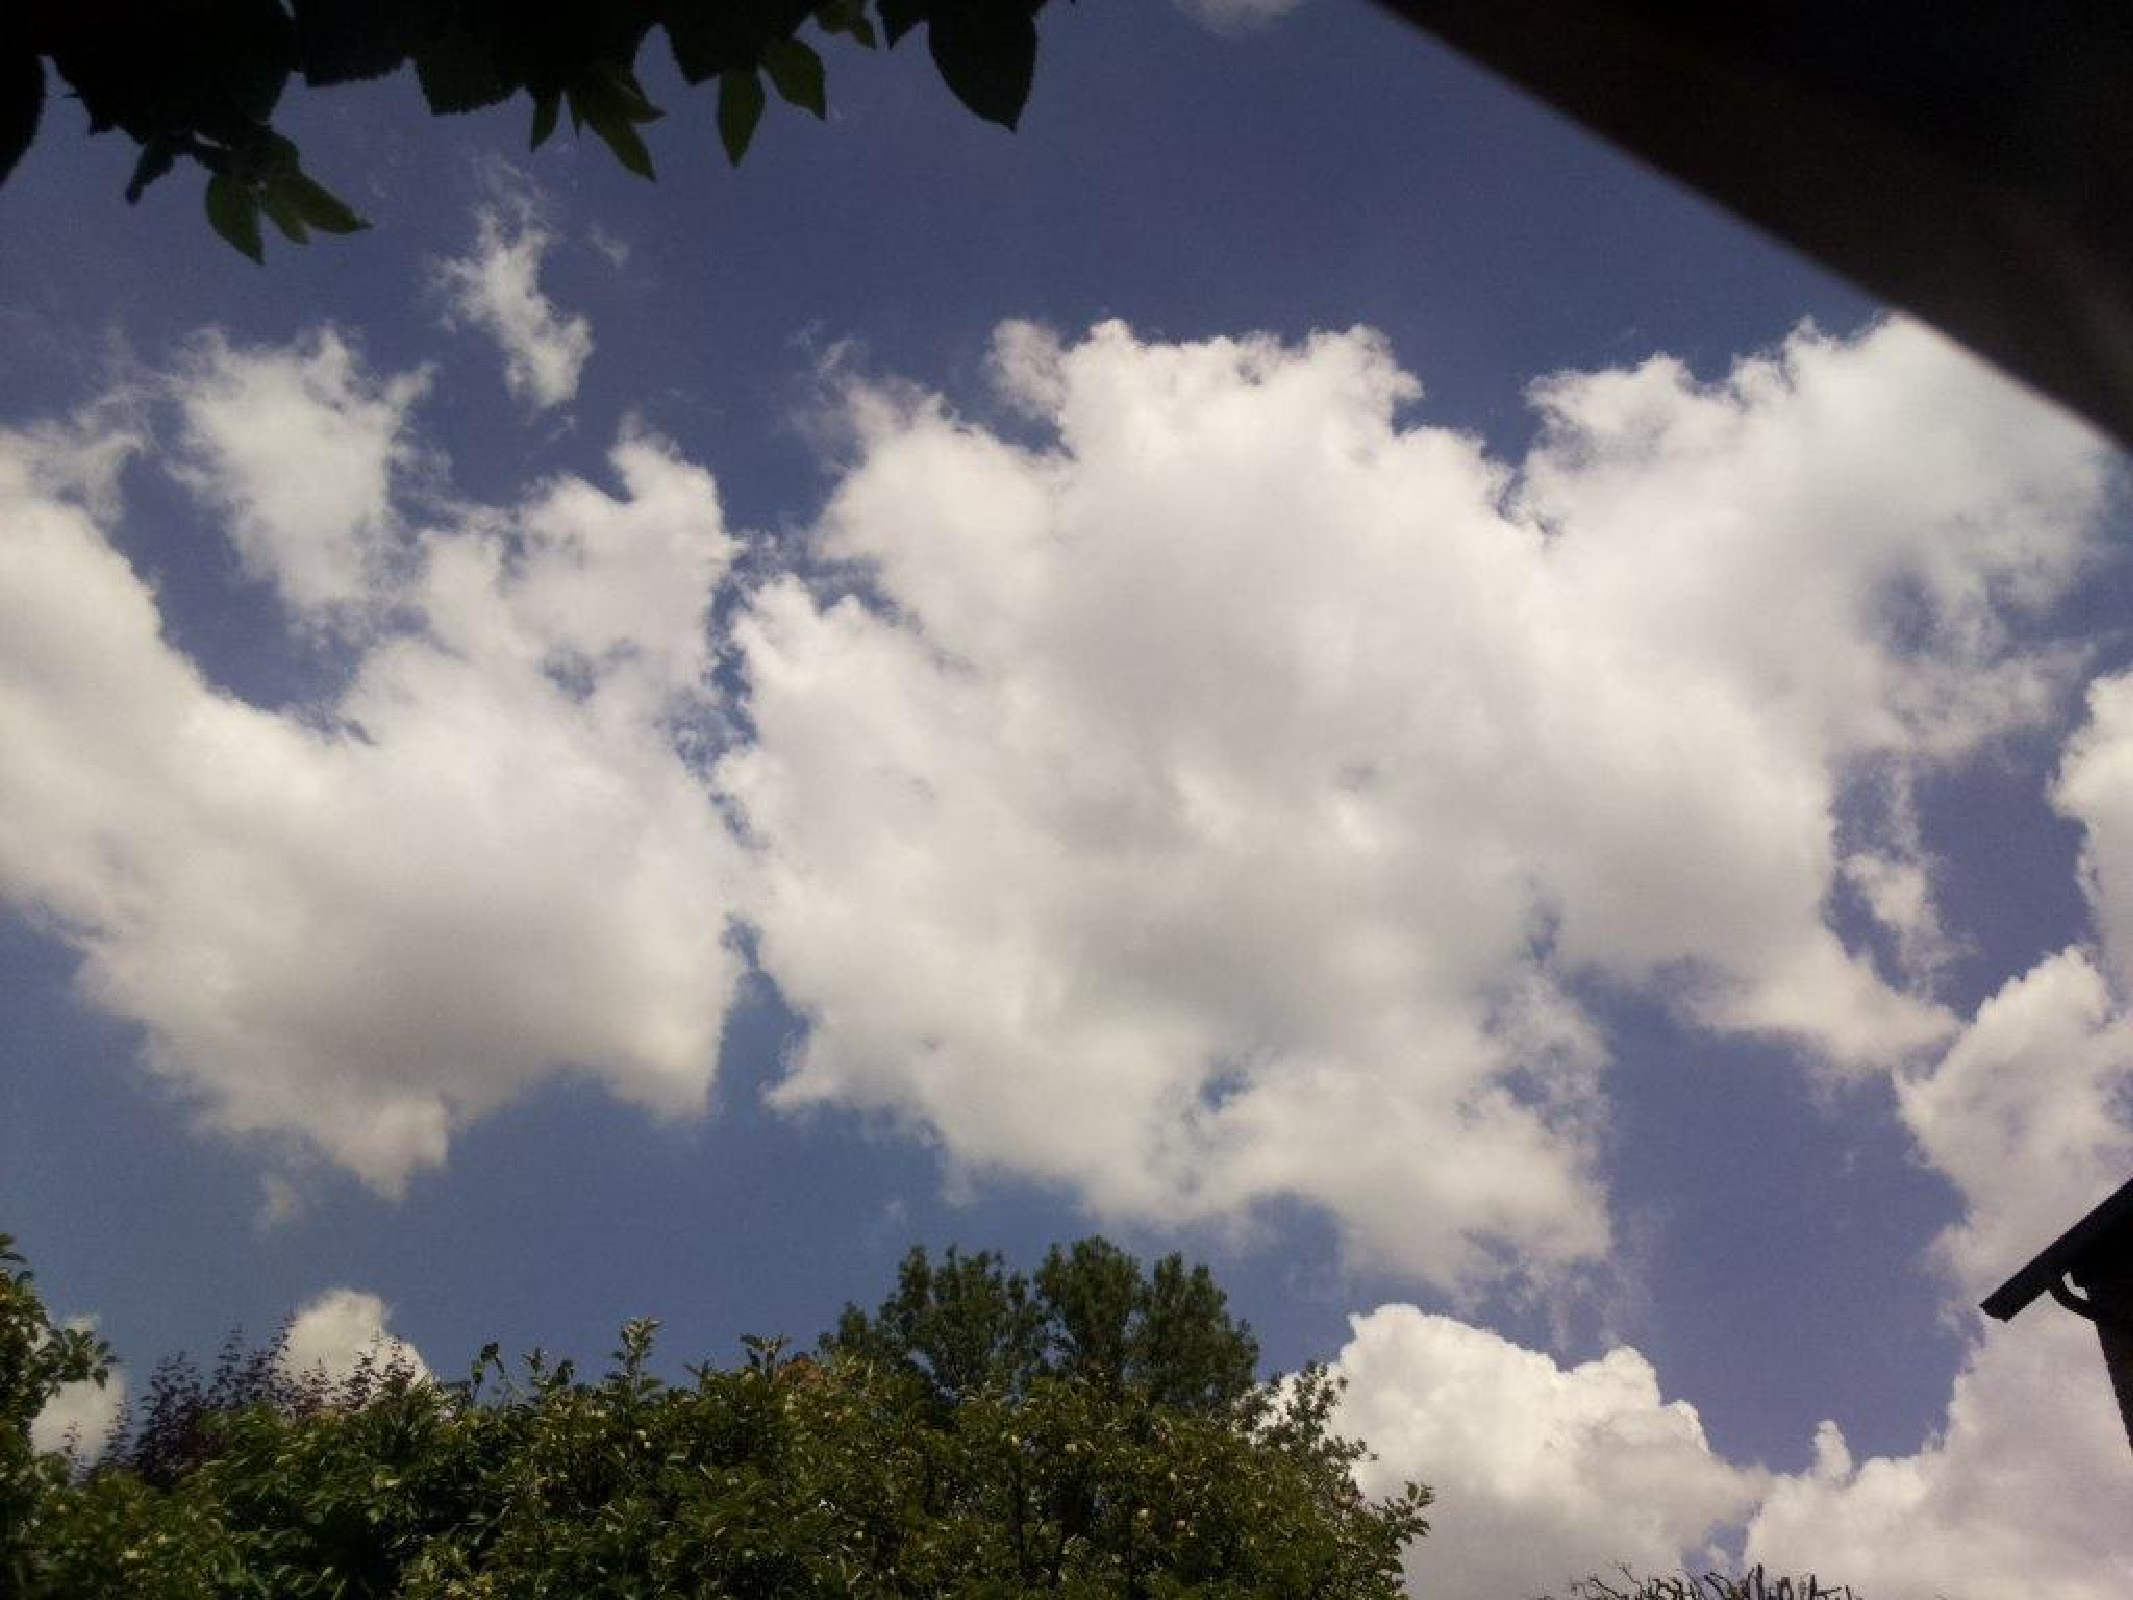
\includegraphics[width=\textwidth]{./pictures/cloudtypes/cumulus.pdf}
		\end{center}
		\caption{Cumulus}
		\label{fig:Cumulus}
		\end{subfigure}
		\begin{subfigure}[b]{0.31\textwidth}
		\begin{center}
				
\includegraphics[width=\textwidth]{./pictures/cloudtypes/nimbostratus.pdf}
		\end{center}
		\caption{Nimbostratus}
		\label{fig:nimbostratus}
		\end{subfigure}
		\begin{subfigure}[b]{0.31\textwidth}
		\begin{center}
				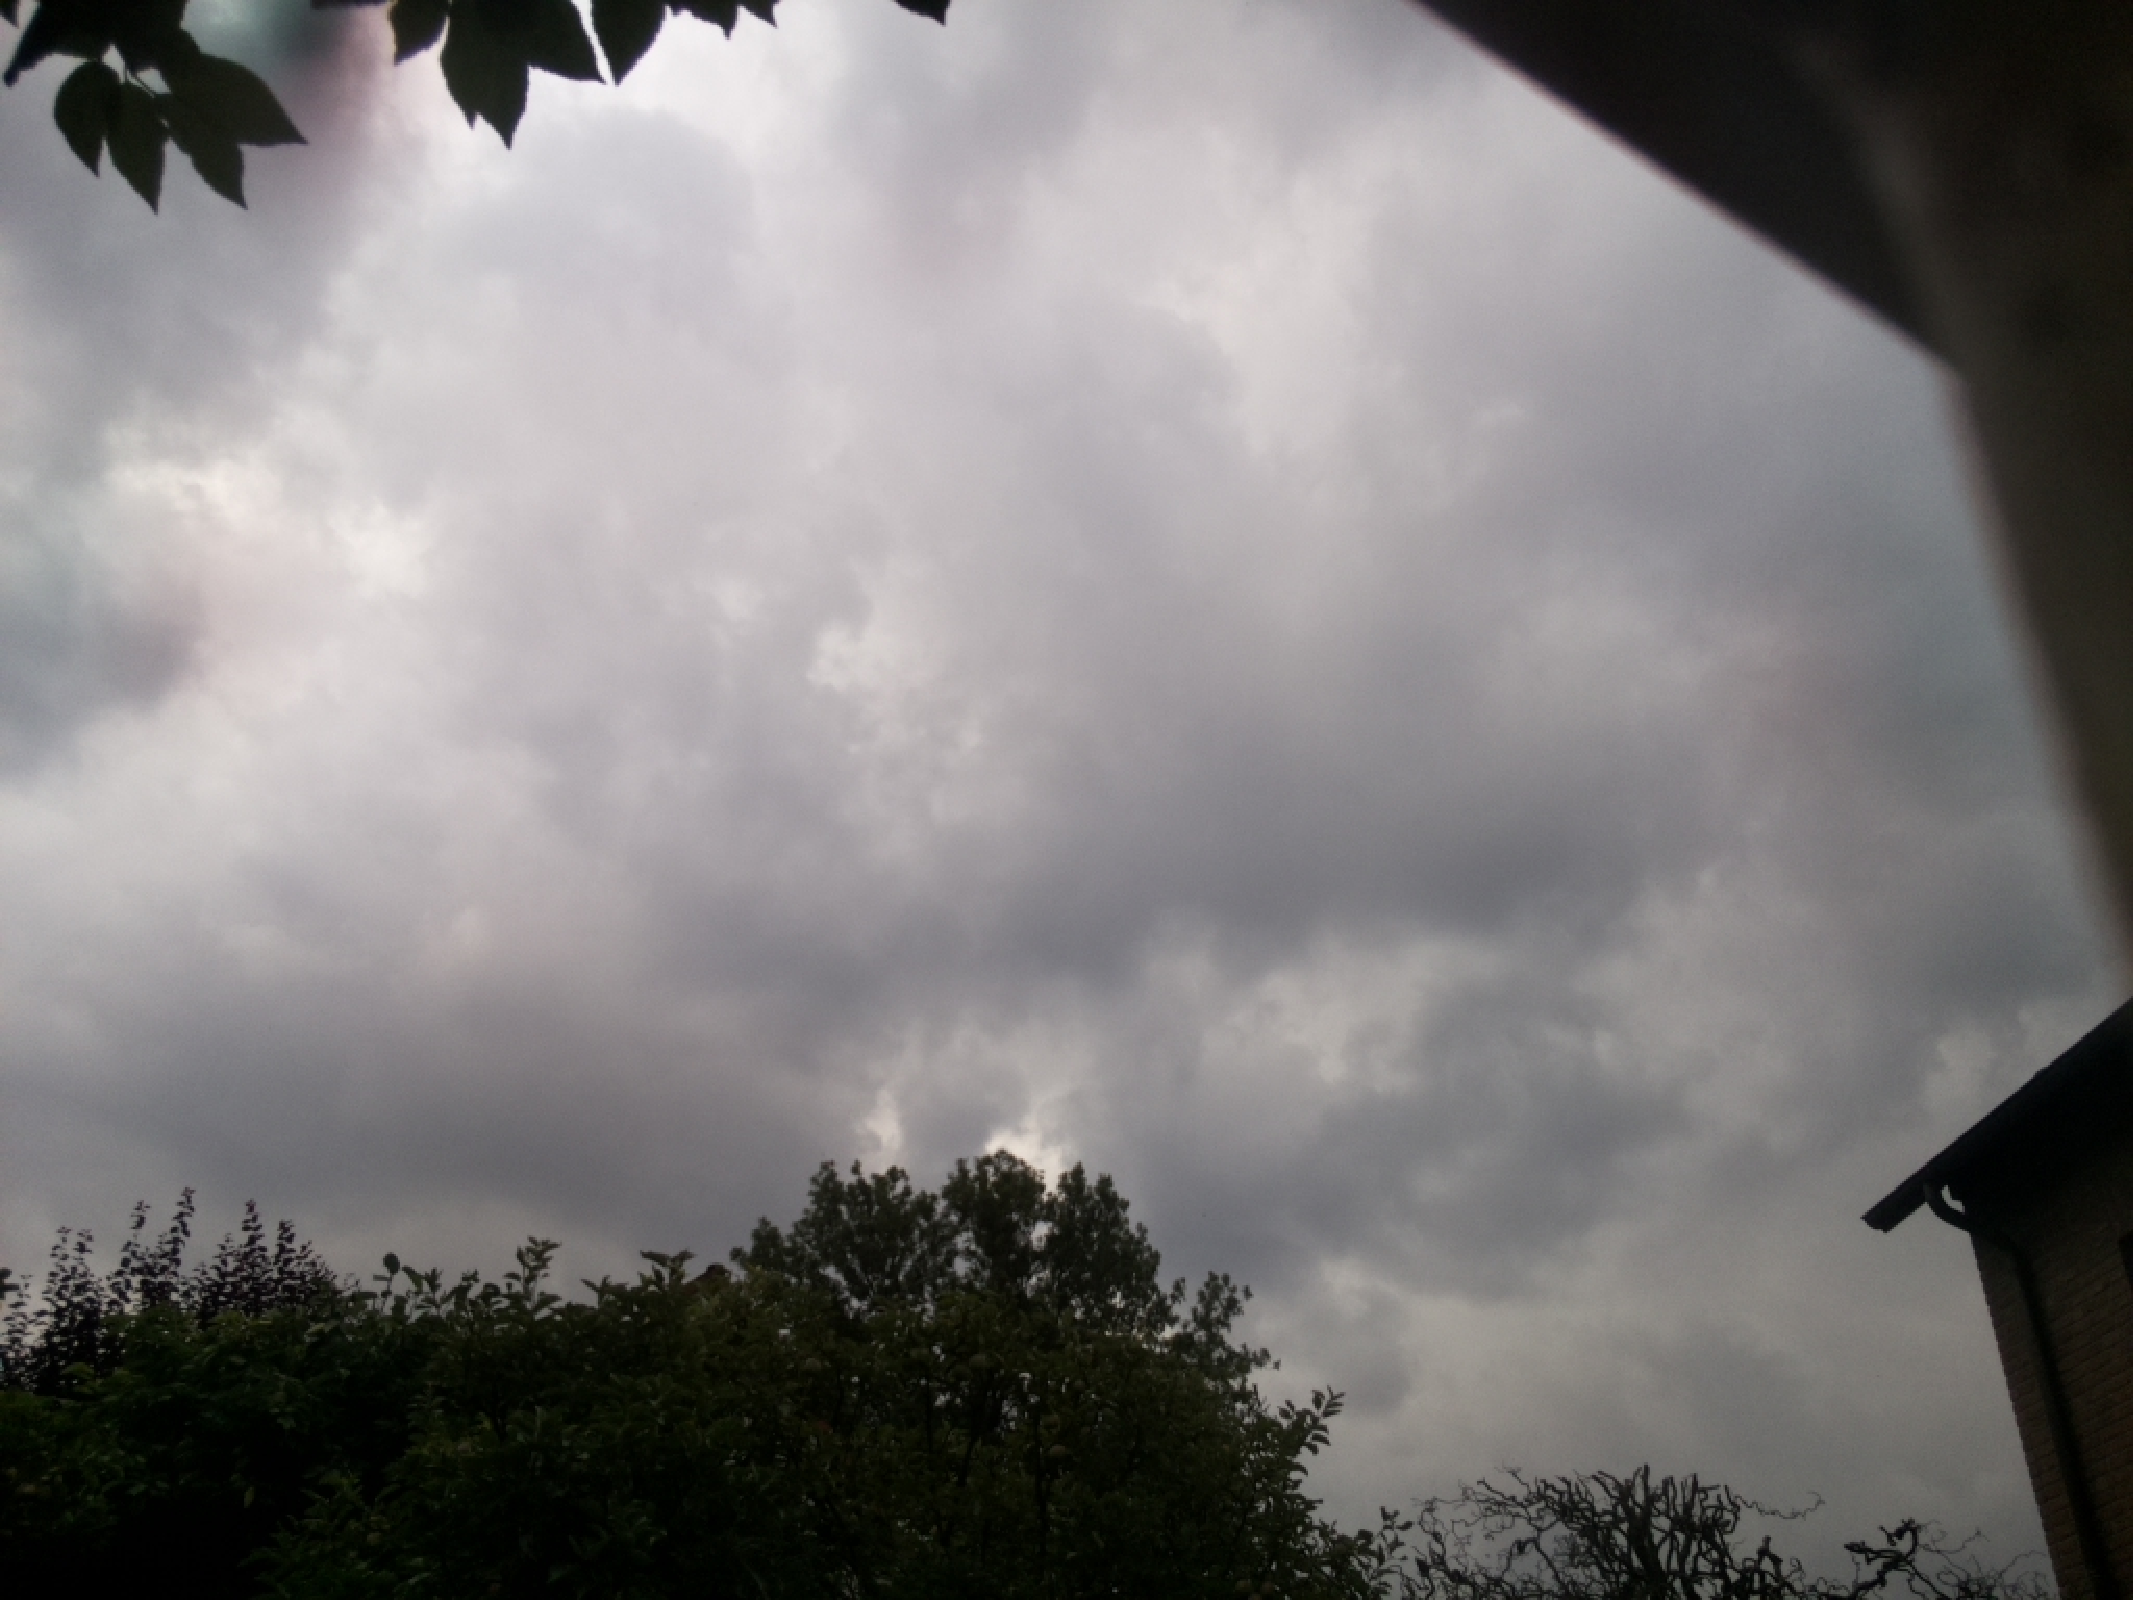
\includegraphics[width=\textwidth]{./pictures/cloudtypes/stratocumulus.pdf}
		\end{center}
		\caption{Stratocumulus}
		\label{fig:stratocumulus}
		\end{subfigure}
		\begin{subfigure}[b]{0.31\textwidth}
		\begin{center}
				
\includegraphics[width=\textwidth]{./pictures/cloudtypes/no_clouds.pdf}
		\end{center}
		\caption{keine Wolken}
		\label{fig:no_clouds}
		\end{subfigure}
		\caption{Repräsentative Fotos für die unterschiedlichen Wolkenklassen.
		Dabei können die Wolkenformen stark variieren. Für umfassendere
		Information können bei dem
		\href{https://telegram.me/weatherpi_bot}{\texttt{TelegramBot}} unter dem
		Punkt \textit{label $\rightarrow$ label $\rightarrow$ info} weitere 
		Informationen angefordert werden.}
		\label{fig:classes}
\end{figure}

\section{Preprocessing}
\label{sec:03_Preprocessing}
Ziel des Preprocessing ist es die Daten aufzubereiten das der
Informationsgehalt maximiert sowie Rauschen minimiert wird.
Desweiteren muessen die Daten so vorverarbeitet werden, dass diese
diese von den machine learning algorithmen ausgewertet werden können. 

Um das Untegrundrauschen zu minimieren koennten Bildausschnitten auf 
denen keine Wolken zu erkennen sind herausgeschnitten werden.
Da das Ziel jedoch eine Möglichst automatisierte Verarbeitung der Date
ist, wird auf die Methode der Farb-Filter zurückgegriffe, da dabei keine
manuelle Nachbearbeitung der Fotos, zur Trennung von Wolken und 
aufgenommener Umgebung benoetigt wird.

Dazu werden Bilder die geringer als \SI{30}{\percent} als die maximale 
Helligkeit besitzen verworfen. 
Durch die Seperation anhand des Helligkeitswert kann anders als Beispielsweise
bei einer Zeitschaltuhr die Messzeit abhaengig von der aktuellen Belichtung 
maximiert werden.
Die Helligkeitsverteilung ist vom Monat als auch von der Wolkendecke abhaengig
ist.
Die Fotos werden noch bevor sie klassifiziert werden der Klasse 'schlechte Fotos' 
zugeordent um den Arbeitsaufwand geringer zu halten.

\begin{wrapfigure}{r}{0.5\textwidth}
		\centering
		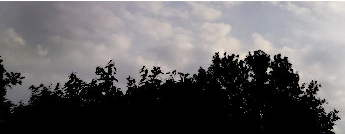
\includegraphics[width=0.45\textwidth]{pictures/cut_out.pdf}
\caption{Anhand des Farbspektrums geschwärzter Untergrund}
\label{fig:}
\end{wrapfigure}
Das Wolkenspektrum hatt klar definierte Farben die Hauptsächlich aus Blau, Grau
und Weiß Tönen besteht. .
Pixel die nicht zu diesem Spektrum gehörsn werden systematisch auf den
Minimalwert gesetzt.
Dazu wird in dem RGB-Farbraum eine Parabel gelegt die Pixel verwirft, die die
Ungleichung 
\begin{equation}
		b > (c - x_0)^2 + x_1
\end{equation}
nicht erfüllen und anschließend die Parabel um die Achse gedreht.
Der Nullpunkt der Parabel wird mit den Helligkeitswerten verschoben.
Ein Beispiel ist fuer Alle  drei Kanäle in Abbildung \ref{fig:??} zu sehen.
Dadurch laesst sich ein grossteil der nicht wolken durch eine Farbe ersetzen.
\begin{figure}
		\centering
		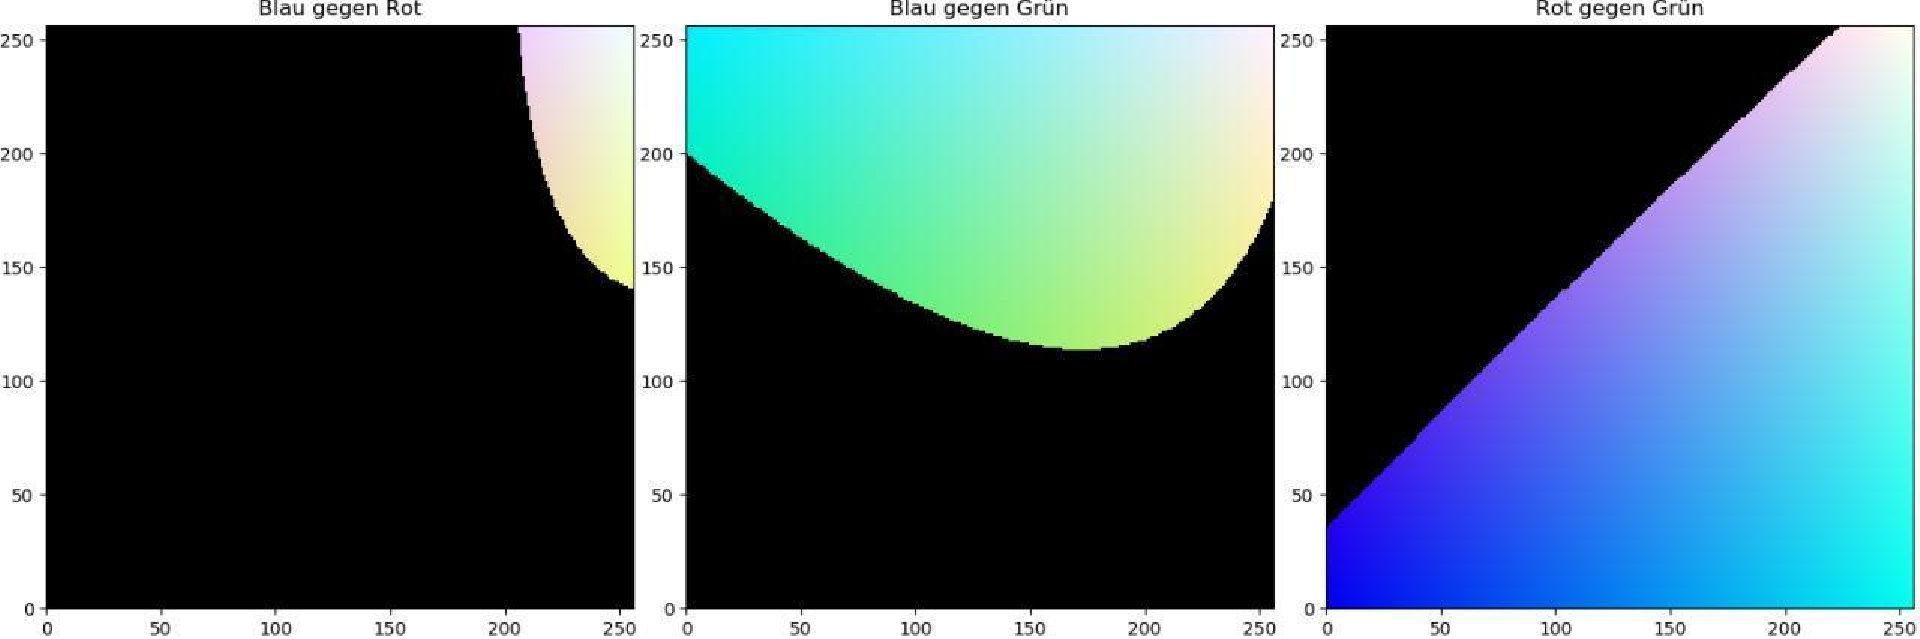
\includegraphics[width=0.8\textwidth]{pictures/colorcube.pdf}
		\caption{Schnitte orthogonal zu den Drei Achsen des RGB-Farbraums fuer den maximalwert.}
		\label{fig:name}
\end{figure}

Nachdem die Daten entsprechend aufbereitet wurden mussen sie noch in Form fuer
die Algorithmen gebracht werden. 
Dazu wird der Farbraum fuer den Random Forrest diskretisiert.
Es bewahrte sich als gut 30 bins pro Farbkanal zu verwenden.
Fuer das Neuronale Netz werden die Bilddaten auf eins normiert.

\section{Machine Learning}

Zur automatischen Bestimmung des Wolkentyps werden zwei verschiedene Algorithmen
verwendet. 
Einer von diesen ist der Random Forest weil dieser out of the box hinreichend schnell,
in der Auswertung und resourcendschonen ist.
Desweiteren wird ein CNN benutzt da dieses in der Laage ist auf den Wolkenformen
sowie dem Farbspektrum zu lernen. 

Beim training der Algorithmen stellte sich heraus das die Daten aufgrund des im
Kapitel \ref{sec:??} beschriebene Problem ein grossen Missmatch aufweisen. 
Daher aendert sich die Zielstellung bei der optimierung wesenltich.
Ziel ist vorerst nicht einen moeglichst hohe Genauigkeit zu erlangen um die
Wolkenklassifikation auf den PIs voran zu treiben sondern den Datensatz zu
erweitern und den Missmatch zu minimieren.
Dazu werden die Methoden genutzt um die Wolken welche nicht mit dem aktuellen
Label uebereinstimmen mittels dem Telegram Bot erneut zu ueberbruefen.
Desweiteren wird bei dem labeln neuer Daten immer ein Label vorgeschlagen
welches ubernommen oder per Hand gelabelt werden kann.
\begin{figure}
		\centering
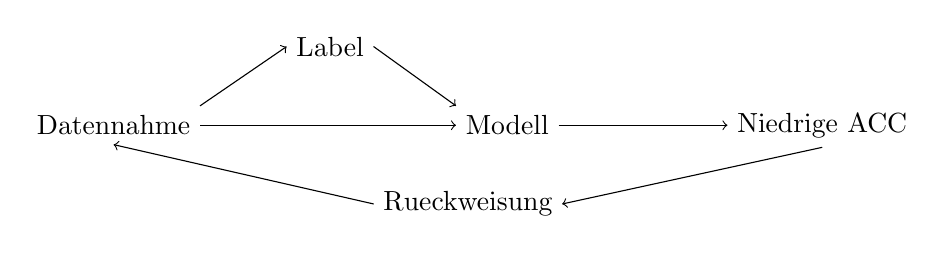
\begin{tikzpicture}[node distance=4cm]
	\node (A) {Datennahme};
	\node (B) [right of=A, xshift=-1.25cm, yshift=1cm] {Label};
	\node (C) [right of=A, xshift=1cm] {Modell};
	\node (D) [right of=C] {Niedrige ACC};
	\node (E) [below of=C, yshift=3cm, xshift=-0.5cm] {Rueckweisung};
	\draw [->, right of=A] (A.north east) -- (B.west);
	\draw [->] (B.east) -- (C.north west);
	\draw [->] (A) -- (C);
	\draw [->] (C) -- (D);
	\draw [->] (D.south) -- (E.east);
	\draw [->] (E.west) -- (A.south);
\end{tikzpicture}
		\caption{Modell fuer weiteres Vorgehen.}
		\label{fig:}
\end{figure}

Selbstverstaendlich bleibt das Optimierungskriterum die ACC wobei abgeleitete
Groessen wie der Loss oder confidence Werte kritisch bei Daten welche einen
Missmatch haben zu betrachten sind.

\subsection{Random Forest}%
\label{sub:random_forest}
\begin{wrapfigure}{r}{0.5\textwidth}
		\centering
		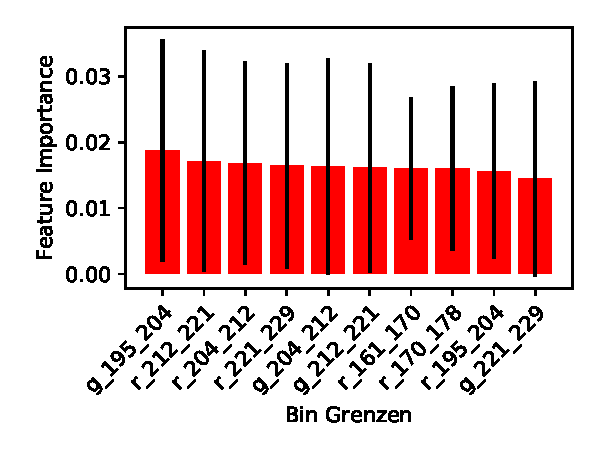
\includegraphics[width=0.5\textwidth]{./pictures/train_rf.pdf}
		\caption{}
		\label{fig:}
\end{wrapfigure}
Fuer das Training des Random Forrest koennen mehrere Parameter variiert werden.
Neben der Tiefe, der Anzahl an gezogenen Feature kann die Anzahl an
Entscheifungsbaeumen varriert werden.
Da die Methode des Random Forest jedoch durch einien hohe Anzahl an Baeumen
gegen Overfitting geschuetzt werden, werden die Tiefe der Baeume nicht weiter
beschraenkt und die Anzahl an gezogenen Featuren nicht weiter optimiert.
Desweiteren ist der histogrammierte Datensatz mit 30 bins pro Farbkanal fuer
machine learning algorithmen sehr niederdimensional.

\subsection{Convolution Neuronal Network}%
\label{sub:convolution_neuronal_network}

Die optimierung des Netzes steht unter der permisse die Architecture des Netzes
so einfach zu halten das die ACC maximal wird und die Parameteranzahl welche mit
der auswertungszeit correllieren kann gering bleibt. 
Beim Training mit der 'Cross Entropy' als Validation loss stellt sich wider
erwarten heraus das der validation loss bei guten Vorhersagen bei einem
Datensatz mit einem Missmatch steigt. 
Dies liegt daran wenn zum Beispiel bei dem waren label A der Datensatz das label
B hat. 
\begin{equation}
		H(p,q) = -\sum_x p(x) \log q(x)
\end{equation}
Somit wird die wahrscheinlichkeit $q(B)$ klein und die Kreuzentropie Gross.
Dies hat zur Folge das die Kreuzentropie bei Datensaetzen mit einem Missmatch
bei der Validierung fuer hohe ACC nicht abnimmt sondern groesse als zum Beispiel
beim Raten ist.
Das Uebertraining kann durch eine loss funktion welche nicht so sensible auf
Missmatches ist. 
Desweiteren wird im Rahmen der Moeglichkeiten der Missmatch der daten zu
minimieren.

\begin{figure}[h]
		\centering
		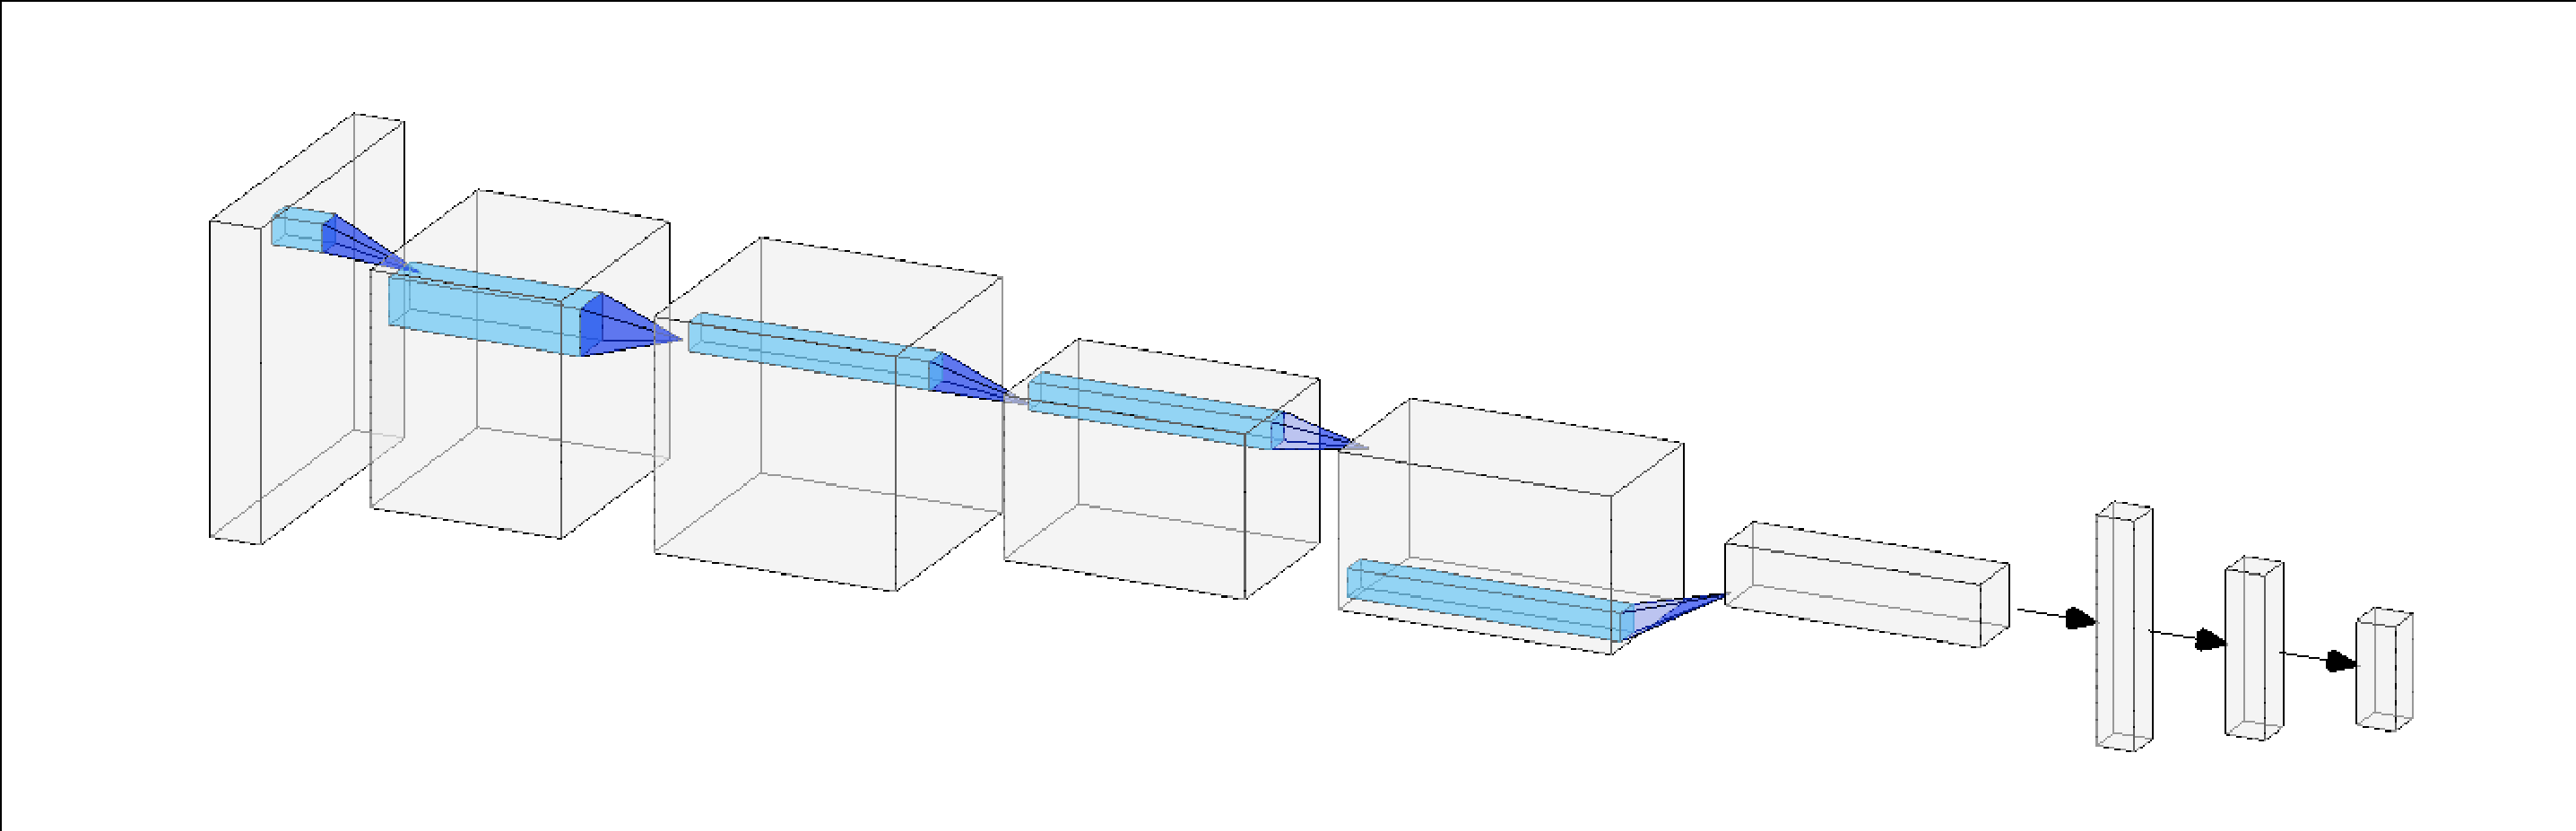
\includegraphics[width=0.8\textwidth]{pictures/architecture.pdf}
		\caption{}
		\label{fig:}
\end{figure}

Als architectur wird zunächst eine AveragePooling schicht gewählt um die
Dimesonalität des Bildes zu verringern.
Anschließend folgen drei Convolution Schichten die der Faltung des Bildes
dienen. 
Zwischen den Convolution schichten werden die Dimesonalität durch jeweils einer
MaxPooling Schicht verringert. 
Anschließend folgen zwei Dense Schichten die der Verarbeitung der
hochdimensionalen Daten dient. 
Diese werden durch jeweils einer Dropout und Noise Schicht regularisiert. 
Abschließend folgt eine Dense schicht mit der Anzahl an neuronen der
Zielklassen.
Fuer die Kernel sowie die Dens schichten wird die Relu funktion als
Aktivierungsfunktion genutzt.
Fuer die letzte Schicht wird entsprechend die Sigmoid funktion verwendet um die
Vorraussagen glatt zu machen und auf 1 zu normieren.

\section{dokumentation interpretation ergebnisse}
\label{sec:04_dokumentation_interpretation_ergebnisse}

Beide Modelle wurden nicht mittels einer Gridsearch optimiert, da durch die
sukssesive Veraenderung der Daten eine aufwendige suche der optimalen Parameter
notwendig waere.
Stattdessen wurde der Fokus auf eher robuste Modelle gelegt die resistente gegen
den Missmatch in den Daten sind.

Der Random Forest erwies sich bei kleinen Datensaetzen und sehr grossen
Missmatchen \SI{30}{\percent} als zuverlaessigeres Modell.
Trotz des Missmatches betrug die Accuracy \SI{50}{\percent}. 
Dies laesst sich darauf zurueckfuehren das der Missmatch mit der relativen
haeufigkeit der Klassen correliert ist. 
Zu den hauefigsten Klassen zaehlen die Klassen 'keine Wolken', 'stratocumulus',
'nimbostratus'. 
Diese weisen alle ein characteristisches Farbspektrum auf und sind einfach
anhand dessen von den anderen Klassen zu trennen.
Das training des CNN dagegen stellte sich als schwierig heraus. 
Trotz verschiedener Kernel-Groessen und anzahl an Convolutional Schichten lies
sich die Accuracy nicht wesentlich uber \SI{30}{\percent} anheben. 
Denkbar waere gewesen auf die Convolution zu verzichten und ebenso wie beim
Random Forest auf dem Farbspektrum zu trainieren.
Dies Methode erschien wesentlich einfacher zu regularisieren und den Missmatch
zu handeln.
Die Entscheidung viel jedoch bewust dagegen aus um das Verhalten des Neuronalen Netzes
auf schlecht simulierten Daten zu studieren. 

\begin{wrapfigure}{r}{0.5\textwidth}
		\centering
		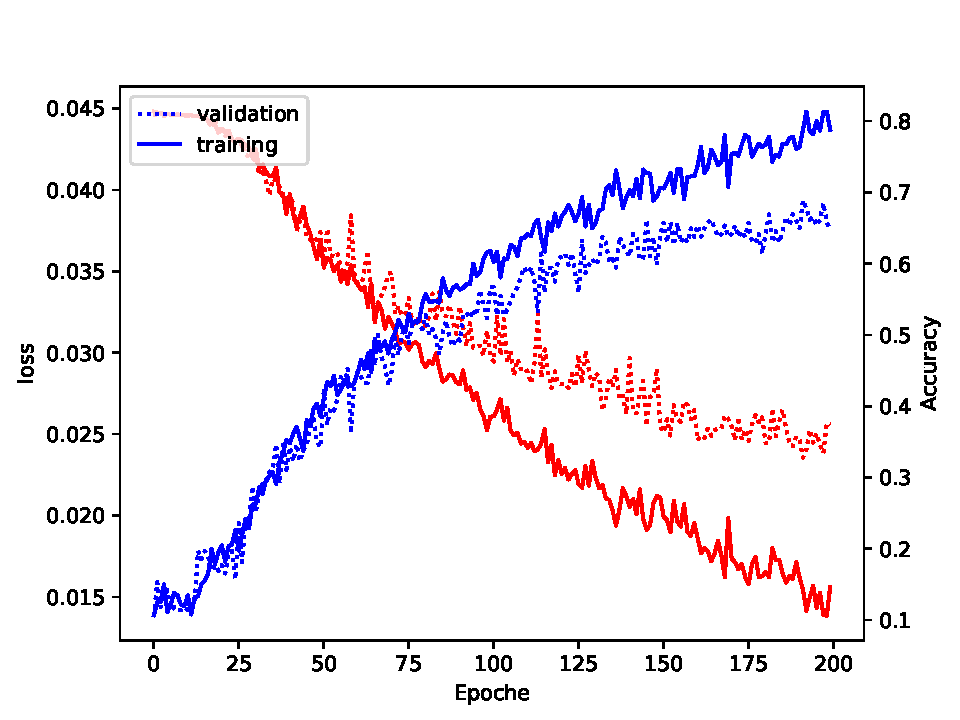
\includegraphics[width=0.5\textwidth]{pictures/train_nn.pdf}
		\caption{Loss sowie Accuracy in Abhaenigkeit der Trainingsepochen fuer
		Trainings sowie validierungsdaten.}
		\label{fig:}
\end{wrapfigure}
Der Random Forrest erreicht auf dem finalen Datensatz der immernoch einen
kleinen Missmatch enthaelt aus der uneindeutigkeit der Klassen und dem Fehler
des Bots eine ACC von \SI{62}{\percent}. 
Auf dem selben Test Datensatz zur evaluation betraegt die Accuracy des CNN
\SI{64}{\percent}.
Dabei ist die Accuracy abhaengig bei welcher Epoche der Schnitt zwischen Over-
und Underfitting macht.
Plausibel erscheint ein schnitt zwischen der \num{70} und \num{85} Epoche.
Auffaellig ist das der Validationloss anschliessend wieder Stark steigt und kein
Platto bildet.
Eine moegliche Ursache koennte der Missmatch seien.
In Abbildung \ref{fig:conf} sind die Confusion Matrizen der beiden Modelle
dargestellt. 
\begin{figure}[h]
		\centering
		\begin{subfigure}[b]{0.49\textwidth}
				\begin{center}
						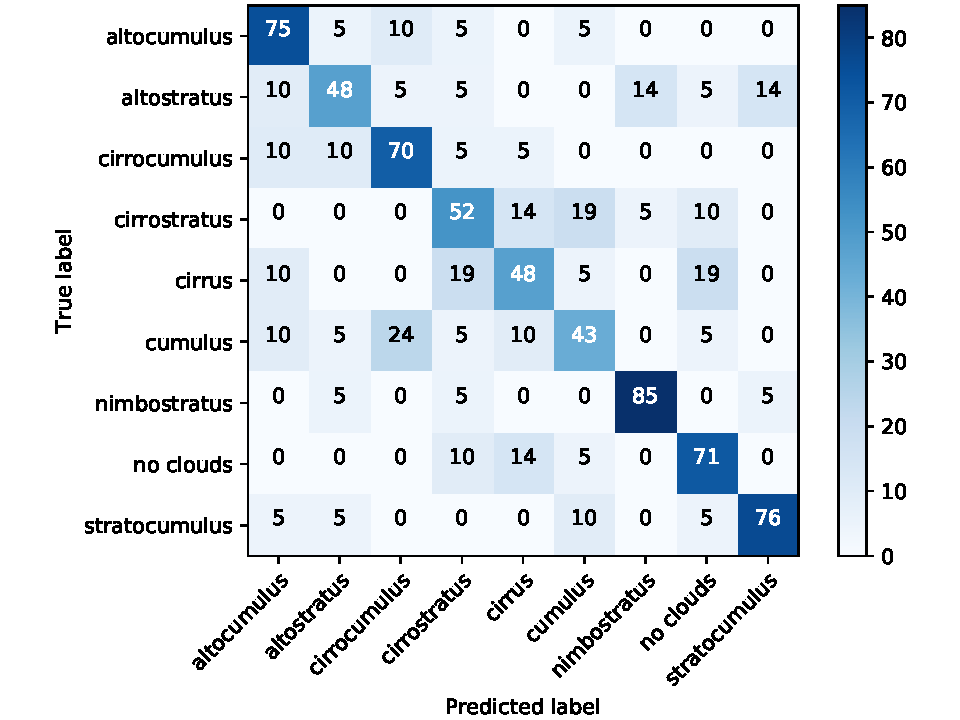
\includegraphics[width=\textwidth]{./pictures/conf_rf.pdf}
				\end{center}
				\caption{Random Forest}
				\label{fig:conf_rf}
		\end{subfigure}
		\begin{subfigure}[b]{0.49\textwidth}
				\begin{center}
						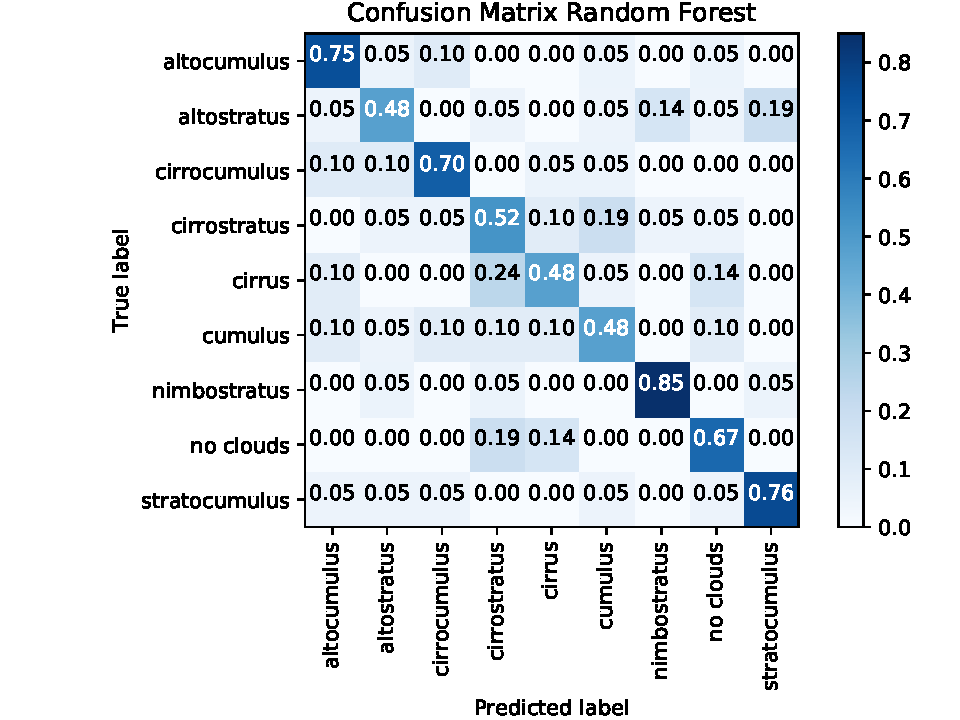
\includegraphics[width=\textwidth]{./pictures/conf_cnn.pdf}
				\end{center}
				\caption{Convolutional Neuronal Network}
				\label{fig:conf_cnn}
		\end{subfigure}
		\caption{Konfidenz Matrizen der observierten Klassen bei denen das
		Vorhergesagte gegen das Wahre Klasse aufgetragen ist.}
		\label{fig:conf}
\end{figure}
Prinzipell scheinen der Random Forrest jeweils Probleme wenn das Farbspektrum
zweier Klassen sich nicht wesentlich unterscheidet.
Dies ist ueberwiegend dann der Fall wenn die Wolkenbedeckung des Himmels sich
Flaechenmaessig aehnelt. 
Beim CNN ist dies \ldots der Fall.

\begin{wrapfigure}{r}{0.4\textwidth}
		\centering
		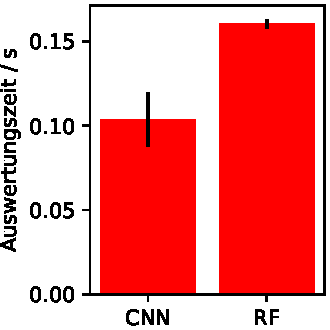
\includegraphics[width=0.4\textwidth]{pictures/time.pdf}
		\caption{Auswertungszeit auf Testdaten der Modelle RF und CNN.}
		\label{fig:}
\end{wrapfigure}
keine Aussage ueber die Trainingszeit.
Zeitlicher vergleich der Methoden.
Wenn moeglich auch die Resourcen.


\section{Zusammenfassung}
\label{sec:05_zusammenfassung}
Mit Hilfe eines \texttt{TelegramBot}s konnten die selbst aufgenommen
Daten gelabelt werden.
Dabei unterlief ein Fehler, sodass die Klassenzugehörigkeit der Bilder teilweise
falsch eingetragen wurde.
Das neugesteckte Ziel ist eine starke Generalisierung der maschinellen Lernern 
um das Training auf den Daten die einen Missmatch haben zu ermöglichen.
Desweiteren konnte das Verhalten der Algorithmen bei einem Datensatz
mit einem Missmatch studiert werden.
Die Trainierten Modelle wurden dazu verwendet den Missmatch 
suksessive zu verringern.
Desweiteren wurde ein Farbfilter sowie die Möglichkeit einen 
Datensatz per Chat zu labeln geschaffen.
Es wurde durch Varation der Architectur versucht das Netz der Problemstellung
anzupassen und die Parameter geschickt zu wählen.
Die Vorhersagegenauigkeit der Modelle sind mit dem Missmatch antikorelliert was
den Fokus auf eine weitere Bereinigung des Datensatzes legt.
Der Random Forest erweist sich dabei als das Modell welches mit 
einem kleinen Trainingsdatensatz und Missmatchen besser umgehen 
kann.

In Zukunft soll der Datensatz wesentlich erweitert werden um das 
Training des CNN zu verbessern.
Desweiteren wird geprüft ob, bei einem hinreichend großen Datensatz sowie
Genauigkeit, 
Modelle Wolken mittels dem sliding Window verfahren tracken koennen.
Dabei sind besonders die Größenänderung sowie die Bewegungsrichtung von
besonderem Interesse.
Dies könnte zum Beispiel sowohl die Präzesion der Wettervorhersage, als auch 
die Routenberechnung für Segelflieger verbessern. 
Dazu werden lokale Wolkenvorhersagen benötigt, die durch die Methode
möglicherweise geschaffen werden können.

\newpage
\section{code anhang}
\label{sec:06_code_anhang}
\begin{wrapfigure}{l}{0.4\textwidth}
\dirtree{%
.1 weatherpi.
.2 predictions.
.3 preprocessing.
.4 cutter.py.
.4 examine\_data.py.
.4 prepro\_data.py. 
.4 prepro\_rf.py. 
.4 to\_do.pkl.
.3 predictions.
.2 weatherpi.
.3 Sensor.
.3 TelegramBot.
.4 label.pkl.
.4 \ldots .
.2 documents .
.2 \ldots .
}
\end{wrapfigure}
Das Projekt wird mittels der Versioncontrolle \texttt{GitHub} von den Inhabern
Maximilian Sackel
und Noah Biederbeck gepflegt. 
Der Code wurde ueberwiegend in den Programmiersprachen Python und die
Documentation in \LaTeX verfasst.

Auf Anfrage kann die Einsicht gewaehrt werden.
Falls Fehler gefunden werden bitte wir Sie die Email
\texttt{maximilian.sackel@gmx.de} zu kontaktieren, damit diese gefixt werden
koennen.
Ueber Anregungen und Verbesserungsvorschläge freuen wir uns ebenfalls.


\printbibliography{}

\end{document}
